\documentclass{article}

\usepackage[utf8]{inputenc}
\usepackage[spanish]{babel}

\usepackage{caratula}

\usepackage{subcaption}
\usepackage{graphicx}
\usepackage{subfig}
\usepackage{dirtytalk}
\usepackage{enumerate}

\usepackage{amssymb}
\usepackage{mathtools}
\usepackage{amsmath}
\usepackage{amsthm}

\usepackage{algorithm}
\usepackage{algpseudocode}
\usepackage{listingsutf8}

\usepackage{float}
\floatplacement{figure}{h!}

\usepackage{geometry}
\usepackage{fixltx2e}
\usepackage{wrapfig}
\usepackage{cite}
\usepackage{dsfont}

\usepackage[space]{grffile}

\geometry{
 a4paper,
 total={210mm,297mm},
 left=30mm,
 right=30mm,
 top=30mm,
 bottom=30mm,
 }
 
\newtheorem{theorem}{Teorema}[section]
\newtheorem{corollary}{Corolario}[theorem]
\newtheorem{lemma}{Lema}[theorem]
 
\theoremstyle{definition}
\newtheorem{definition}{Definición}[section]
 
\theoremstyle{remark}
\newtheorem*{remark}{Observación}
 
\begin{document}
% Estos comandos deben ir antes del \maketitle
\materia{} % obligatorio

\titulo{Trabajo Práctico 1}
\subtitulo{}
\grupo{}

\integrante{Bayardo Julián}{850/13}{julian@bayardo.com.ar} % obligatorio
\integrante{Cuneo Christian}{755/13}{chriscuneo93@gmail.com} % obligatorio 
\integrante{Fosco Martín Esteban}{449/13}{mfosco65@gmail.com} % obligatorio 
\integrante{Germán Pinzón}{475/13}{pinzon.german.94@gmail.com}
 
\maketitle

\pagebreak

\tableofcontents

\pagebreak

\section{Introducción}

En el presente trabajo se analizan diversos aspectos de la red utilizando Scapy y se distinguen algunos componentes de la misma utilizando un enfoque formalizado a través del uso de la teoría de la información.

En primer lugar, planteamos un criterio para la identificación de routers IPv4 en redes de área local basándonos únicamente en paquetes ARP interceptados de la red.

En segundo lugar, se presentarán cuatro experimentos realizados sobre distintas redes (tres de ellas redes no controladas y una red casera), consistentes en observar el tráfico de las mismas, intentar comprender la topología de la red, y comprobar la eficiencia de el criterio propuesto.

Finalmente, presentaremos las conclusiones y lecciones aprendidas a partir de los mismos.

\subsection{Criterio de distinción}

Primero, recapitulemos sobre el funcionamiento de ARP en una red IPv4. ARP es un protocolo orientado a la resolución de addresses de hardware a partir de addresses IP: cuando un host A pretende comunicarse con otro host B dentro de la misma red de área local, precisa de la MAC address del host B para poder enviar el paquete al destino; de por sí, ningún host poseé esta información sobre ningún otro host y, por ende, precisamos de una metodología para obtenerla.

En el caso de ARP, esto se realiza a través de dos paquetes enviados sobre IP: los ARP Whois y ARP Is At. En el primer caso, el host A precisa saber el MAC address de B, y por ende envía un paquete de este tipo, donde los campos de source de Ethernet e IP serán los de A, y el MAC address destino será FF:FF:FF:FF (address de broadcast para Ethernet), y el IP address de destino será el IP con el que A quiere comunicarse. Luego, todos los nodos dentro de la misma red que reciban el paquete re-enviaran el paquete en todas las otras interfaces en las que aun se encuentren dentro de la red local. La única excepción a esta regla es si la interfaz por la que se recibió el paquete tiene asignada la IP de destino del paquete Whois. En este caso, el host enviará un paquete de tipo ARP Is At, con destination igual al source del paquete anterior, y source con los datos propios del host. Una vez que el host que realizó el Whois recibe el IsAt, tiene la MAC Address del host que estaba buscando en el campo de source.

Pensemos, entonces, en cómo seleccionar un host distinguido basándonos únicamente en los paquetes ARP: tenemos 5 campos posibles para pensar: tipo de paquete, source IP address, source MAC address, destination IP address y destination MAC address. Como los tipos de paquete pueden ser 2, pensemos qué pasa con cada uno de estos campos en ambos casos:

Si el paquete es de tipo Whois, queda claro que el destination MAC address no nos va a brindar ninguna información, ya que está fijado a FF:FF:FF:FF. Por otro lado, el source IP address y source MAC address tampoco lo harán: cualquier host que deseé enviar un paquete IP precisará de estos campos, y por ende tendremos muchos host, donde los que sobresaldrán serán aquellos que busquen muchos destinos. Por otro lado, el destination IP address nos da una buena medida de qué IPs son las más requeridas.

En el caso contrario, tenemos que los destination MAC e IP addresses, junto con source IP address, cumplirán los mismos roles que tenían anteriormente, y por ende la información será la misma, pero el source MAC address ahora si tendrá un valor, que será específicamente el del nodo requerido. Observemos que esto también nos da una medida de "popularidad" entre nodos de la red, de la misma forma en que lo hacía anteriormente el destination IP address (de hecho, asumiendo que no se perdiesen paquetes en ningún momento, y el router tuviera una única IP asignada a la interfaz con ese MAC, deberían darnos la misma cantidad de información).

Con esto en mente, nos pareció relevante elegir como router al nodo cuya IP tenga la menor cantidad de información considerando una fuente que emite los destination MAC address de los paquetes ARP Whois. La idea detrás de esto es la siguiente:

En una red LAN con acceso a Internet, lo más probable es que los host de la LAN tiendan a buscar hosts que estén fuera de la red local, y por ende deban enviar el paquete hacia su default gateway para ser forwarded hacia el proveedor de internet. Esta simple observación nos dice que el router tiene altas probabilidades de ser el host con el que más busquemos conectarnos dentro de la red local; teniendo como posibles contendientes a servidores locales que puedan tener mucho uso (por ejemplo, un servidor DNS corriendo por separado, un fileserver, etcétera). 

\subsection{Aclaraciones sobre la recolección y análisis de datos}

La recolección de datos fue realizada con Scapy según el enunciado del TP, exportados a csv, y procesados con Tableau. Los archivos correspondientes se encuentran en la carpeta raíz del trabajo práctico. Las redes analizadas son, en orden de presentación, la red Wi-Fi abierta Laboratorios-DC de la facultad, la red laboral con medios mixtos de Mercado Libre, la red Wi-Fi abierta del Shopping Dot, la red Wi-Fi abierta de un McDonalds, y una red Wi-Fi casera sobre la que tenemos control. Observemos que las elecciones nos permiten analizar un abanico interesante de combinaciones posibles, aunque lamentablemente la falta de información sobre la topología de la mayoría de las redes sólo nos permite conjeturar.

En términos de la presentación de los datos, debido a la gran cantidad de hosts que encontramos en la mayoría de las redes, fue necesario excluir muchos de estos de los gráficos presentados para que los mismos sean legibles. Para la exclusión, consideramos un corte donde los nodos cuya probabilidad de aparición sea menor a X (dependiente del gráfico) son excluídos. Este filtro fue aplicado sobre todos los gráficos con excepción de la red casera, y la probabilidad X fue de 4e(-4) en todos los casos con excepción de la red de Mercado Libre, donde el corte fue de ligeramente menor.

Esto es relevante debido a que nosotros mostramos marcas para la entropía y promedio de las distribuciones de probabilidad, y queremos aclarar que si bien el promedio está tomado únicamente sobre los datos mostrados en los gráficos, la entropía está calculada sobre el total de la distribución (es decir, es lo que debería ser). Esto es debido a una restricción del software utilizado para graficar, y lamentablemente no encontramos forma de arreglar el problema.

\newpage
\section{Primer Experimento: Laboratorios-DC}

\subsection{Presentación y Suposiciones}

En el siguiente experimento, se analiza la red Wi-Fi del Pabellón 1 de Ciudad Universitaria: Laboratorios-DC. Nos dedicamos a recibir los paquetes de la red durante 30 minutos y guardar los datos relevantes para este experimento sin ninguna clase de filtrado.

Para la primera etapa del experimento, veremos los diversos protocolos que se pudieron observar, suponemos que lo más probable será encontrar paquetes del protocolo IPv4 (ya que la misma no asigna direcciones IPv6 a través de DHCP) y ARP (para aprender la dirección MAC de algún host).

Luego, veremos los nodos involucrados en las comunicaciones del protocolo ARP, es probable que la mayoría de los nodos preguntando direcciones buscan la dirección del Gateway por medio del cual van a poder acceder a Internet.

\subsection{Resultados}

\subsubsection{Protocolos}

\begin{figure}[H]
\centering
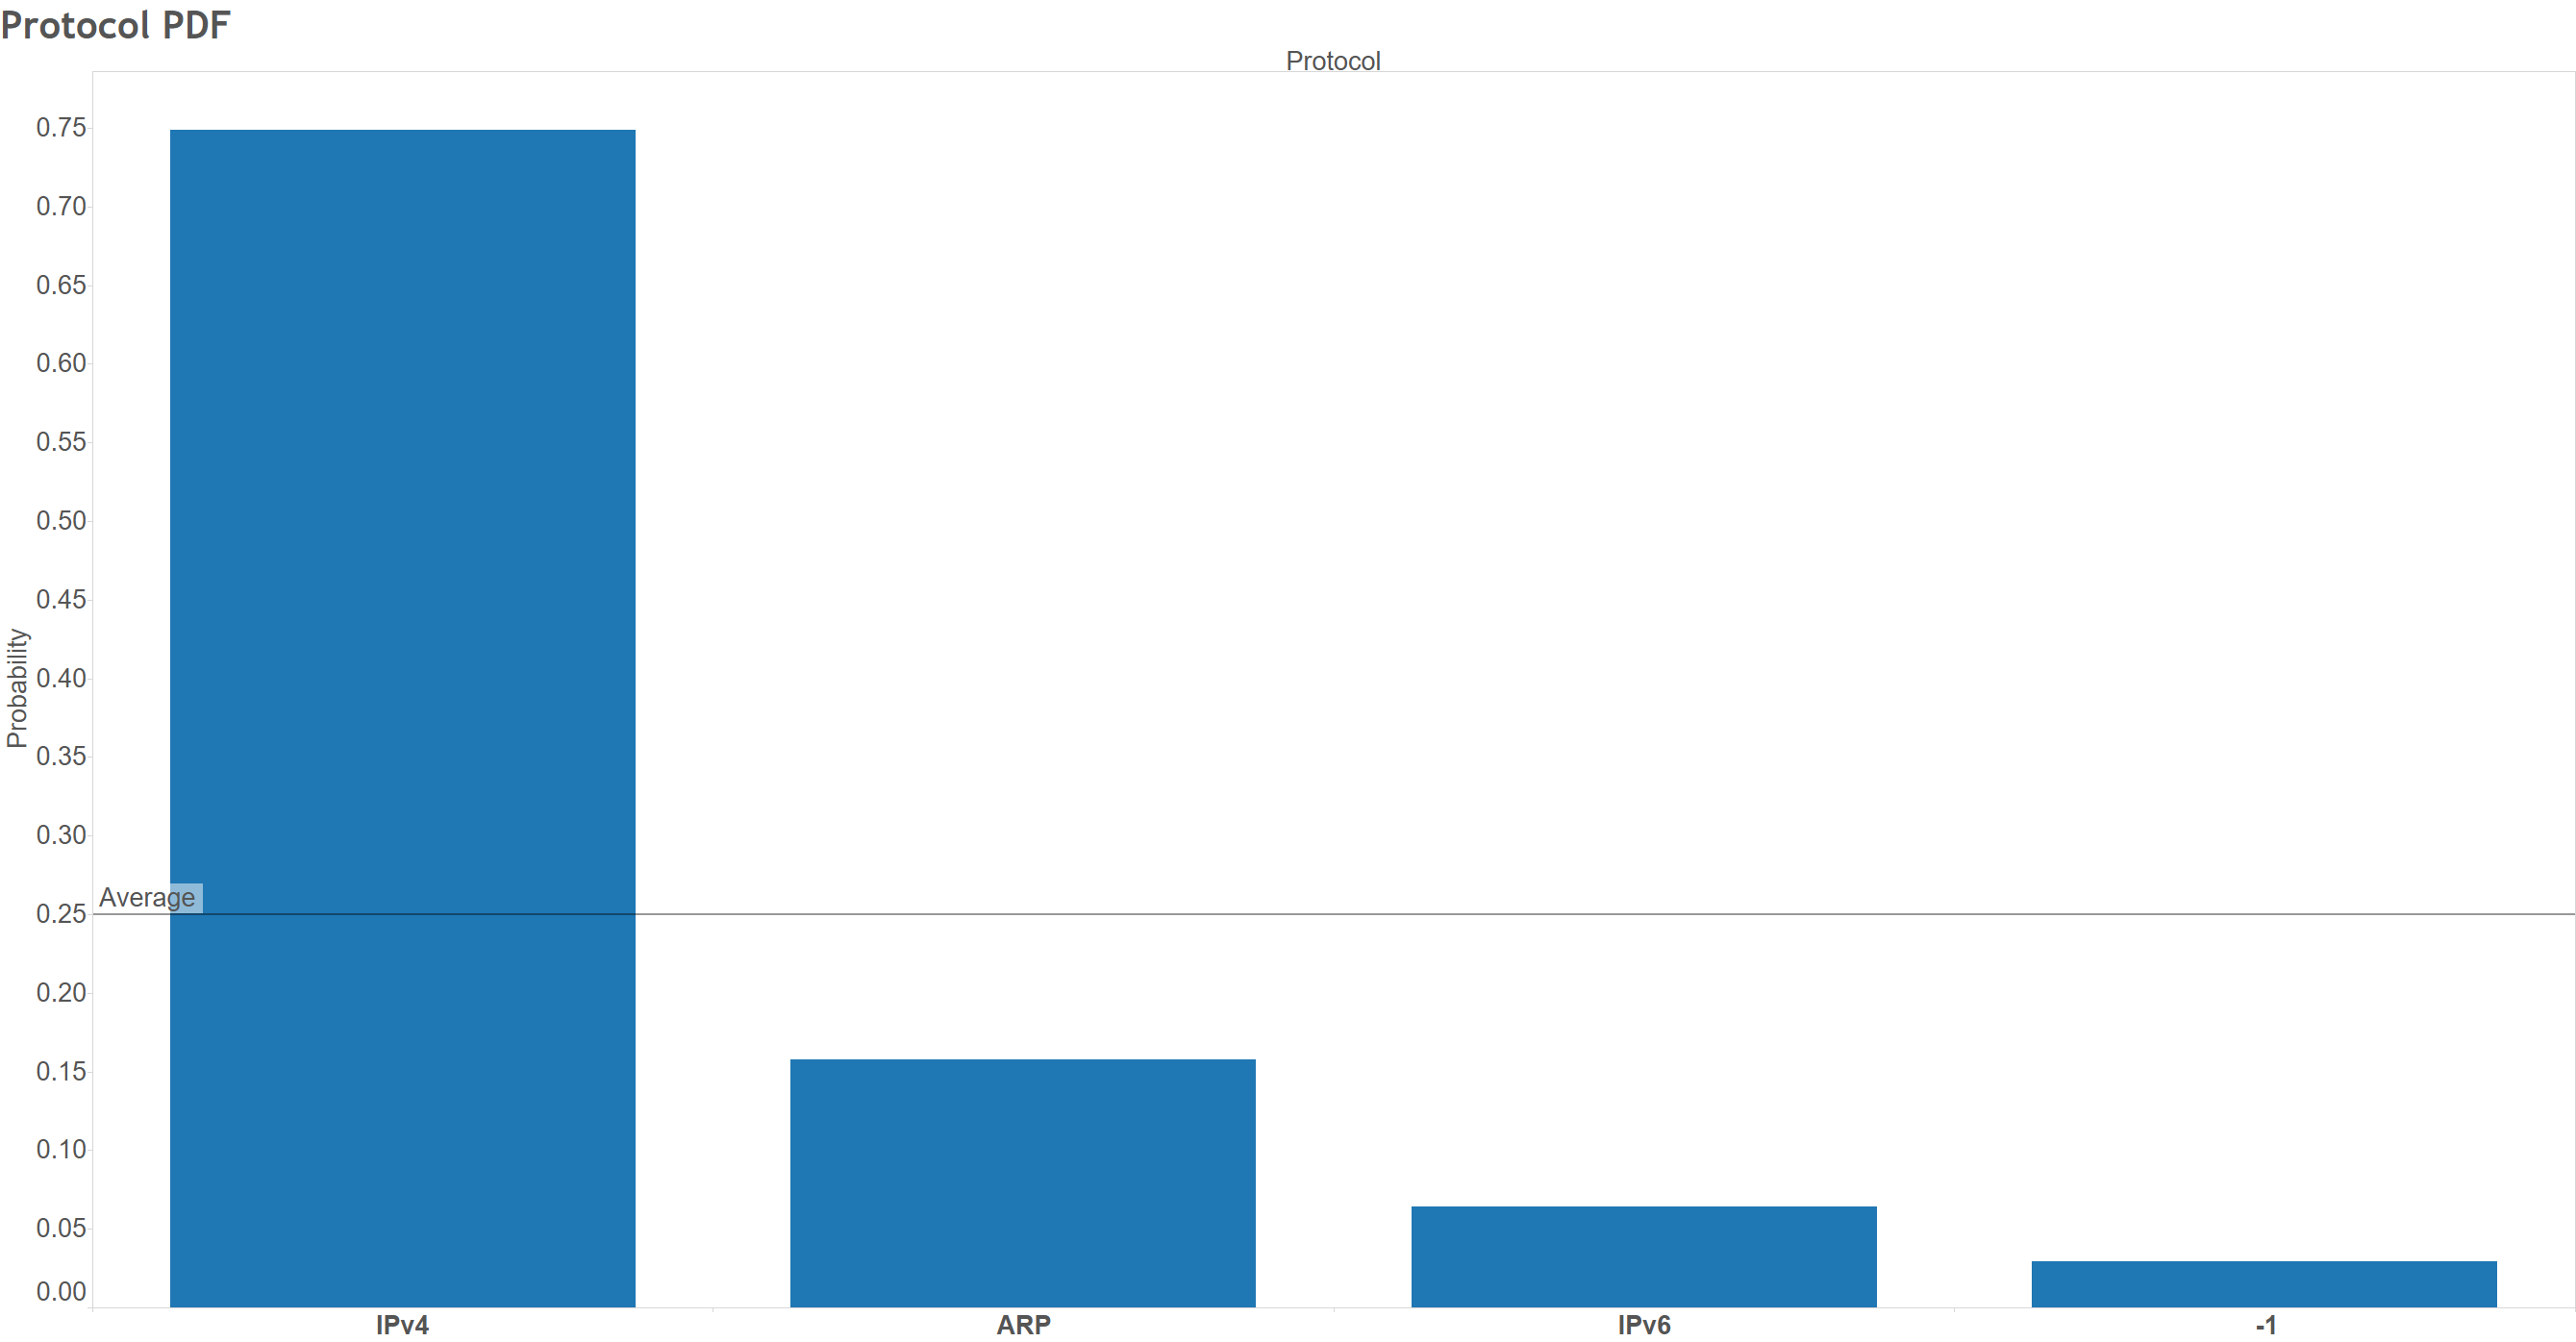
\includegraphics[width=450pt]{captures/LabosDC/Protocol PDF Dashboard Probabilitidad.png}
\caption{Cantidad de información de cada símbolo para una fuente que emite los tipos de protocolos encapsulados, con probabilidad para cada símbolo según estimamos a través de la captura de la red}
\end{figure}

Como habíamos supuesto, IPv4 y 
ARP efectivamente son los tres protocolos con mayor grado de incidencia en la red, sólo basta con ver la distribución de probabilidad estimada a partir de los datos, (que se puede ver también como la distribución del conjunto total de paquetes enviados). Este resultado es completamente esperable, dado que:

\begin{itemize}
\item ARP es uno de los protocolos más necesarios para el funcionamiento de un nodo en una red de este nivel, tanto para actualizaciones periódicas de información pertinente a la red como para obtener la información esencial al momento de conectarse e iniciar las comunicaciones en dicha red.

\item IPv4 es la versión más utilizada para la transmición de información en redes IP.
\end{itemize}

Si bien no nos esperábamos la existencia de tráfico IPv6, encontramos una relativamente pequeña cantidad de tráfico relacionado. Desconocemos el motivo de este tipo de tráfico, ya que como mencionamos anteriormente no hay direcciones asignadas por DHCP.

Procesando los datos anteriores en un gráfico más estrechamente relacionado a los conceptos vistos en clase, si consideramos a toda la red una fuente y a cada emisión con un protocolo distinto un símbolo distinto, entonces obtenemos la siguiente figura:

\begin{figure}[H]
\centering
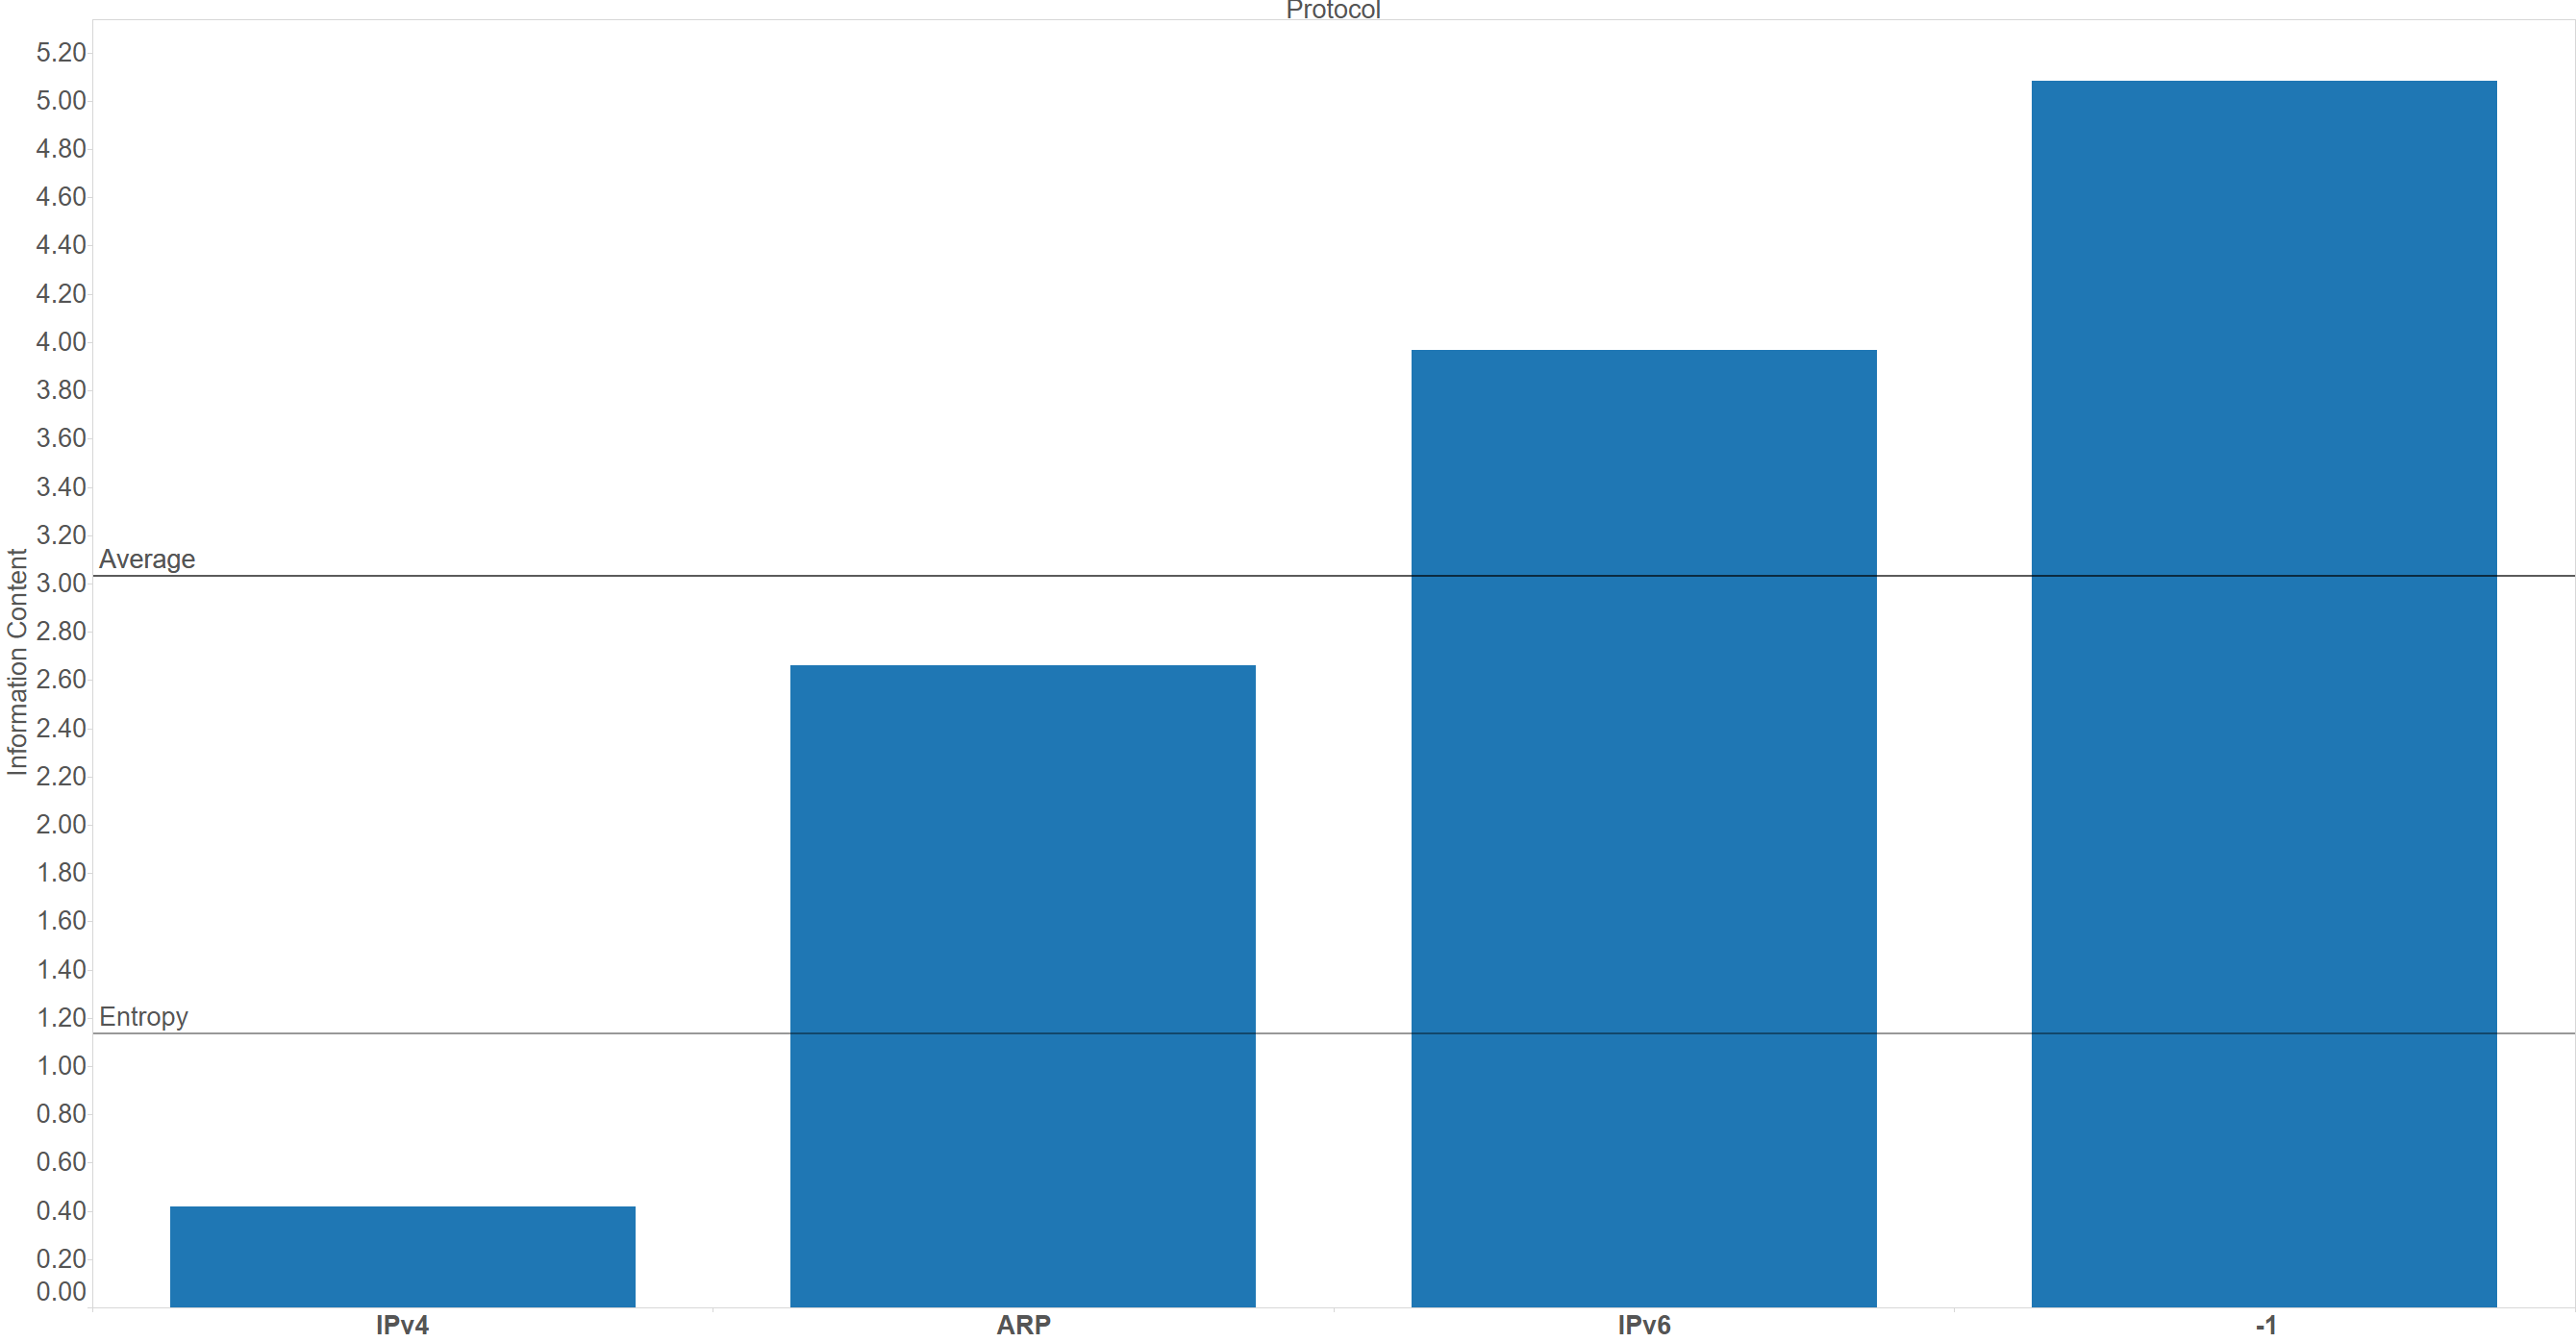
\includegraphics[width=450pt]{captures/LabosDC/Protocol PDF Dashboard.png}
\caption{Cantidad de información obtenida de un paquete de cada tipo de protocolo, -1 representa protocolos distintos a IPv4, IPv6 y a ARP.}
\end{figure}

Evidentemente, al ser más común hallar mensajes de protocolo IPv4, obtendremos menor información de esta clase de mensajes, por otro lado ARP e IPv6 se alejan más de la entropía por su menor incidencia, las apariciones del resto de los protocolos son aún menos frecuentes, por lo que obtendremos una mayor cantidad de información para estos que para cualquier otro.

Podríamos considerar un protocolo distinguido a IPv4, debido a que es el menor (dentro de los 3 que nos interesan) en relación a la cantidad de información que proporciona, es además es más alejado de la entropía (por debajo), en este caso es alejado en el sentido de que recibiríamos una cantidad menor de información de dicha ocurrencia debido a que la ocurrencia de un mensaje de protocolo IPv4 es relativamente común.

\subsubsection{Nodos ARP}

Pasemos ahora a analizar la captura de la red enfocándonos en los nodos de la red que hayan transmitido o enviado datos mediante el protocolo ARP.

\begin{figure}[H]
\centering
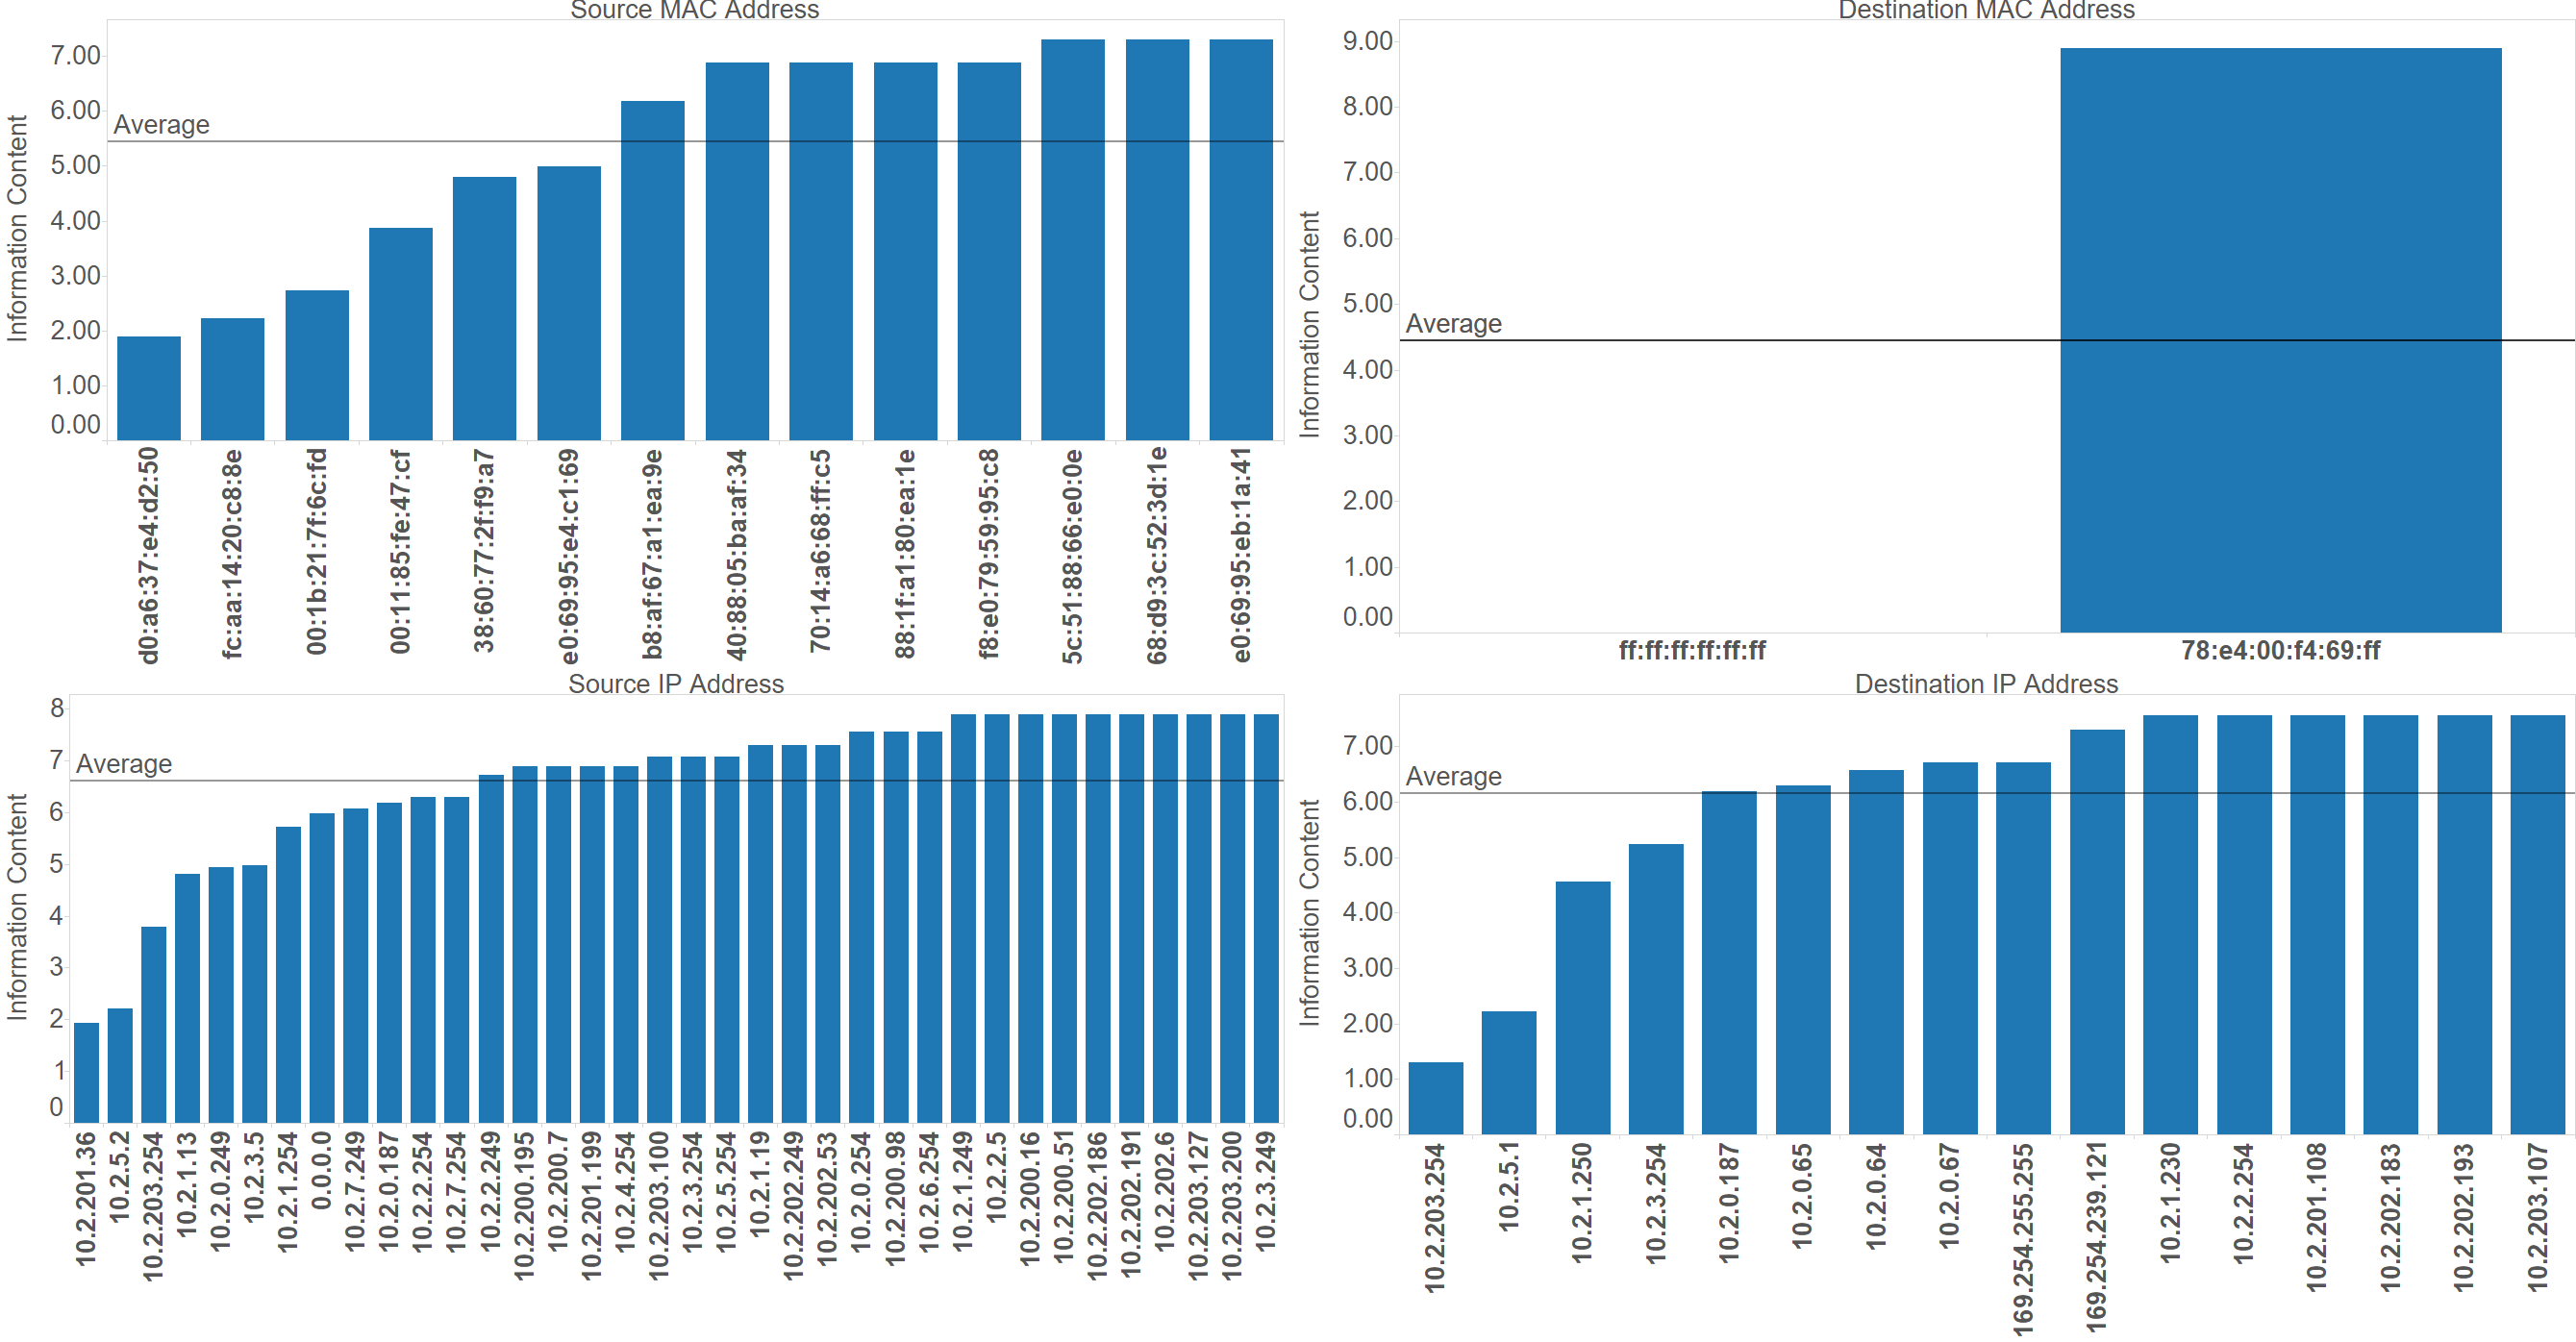
\includegraphics[width=450pt]{captures/LabosDC/PDFs Dashboard.png}
\caption{Para cada gráfico, se muestra en el eje abscisas ponemos los símbolos que consideramos como salida de nuestra fuente de información, y en las ordenadas ponemos la cantidad de información obtenida por la observación del símbolo. Las lineas horizontales muestran el promedio de los valores mostrados, y la entropía de la fuente contemplada, respectivamente.}
\end{figure}

Se pueden sacar en limpio de estos gráficos las siguientes observaciones:

\begin{itemize}
 
\item En \textbf{Source MAC Address} y \textbf{Source IP Address}, encontramos que hay pocos nodos activos (el corte eliminó una cantidad muy grande de nodos con muy poca cantidad de información), y no parece notarse ninguna diferencia particular entre los nodos más activos analizando los datos subyacentes.

\item Por otro lado, en \textbf{Destination MAC Address} se hace evidente una confirmación de lo que habíamos conjeturado en la introducción: la operación con más incidencia es el broadcast que corresponde con un ARP Whois, y por ende tenemos al FF:FF:FF:FF:FF:FF como el address que proporciona menos información.

\item Finalmente, en \textbf{Destination IP Address} podemos determinar como nodo distinguido a 10.2.203.254, que tiene mayor incidencia en destination (es el que más mensajes ARP recibe) y bastante incidencia tiene en source (es uno de los que más mensajes envían). 

\end{itemize}

En conclusión, consideramos como nodo distinguido el nodo 10.2.203.254 porque es el que más incidencia tiene en las comunicaciones del protocolo ARP de la red elegida, en particular aparece más veces en \textbf{Destination IP Adress}, por lo tanto es el símbolo que menor información provee respecto de todos los otros. Efectivamente, corroboramos que este mismo es el que se corresponde con el default gateway según se distribuye por DHCP.

\newpage
\section{Segundo Experimento: McDonalds}

\subsection{Presentación y Suposiciones}

En este experimento, se analizó la red Wi-Fi de un local de McDonalds, recibimos los mensajes circulando por la red durante 20 minutos. Procedemos a presentar y analizar los resultados de manera análoga al experimento anterior.

Estimamos que, como fue el caso también el experimento anterior, deberíamos registrar poco o nada de presencia del protocolo IPv6, y tener al IPv4 como el protocolo más distinguido. Además, pensamos que dado que la red es de acceso público y el local estaba localizado en una zona con alta densidad poblacional, vamos a encontrar una gran cantidad de nodos conectados.

\subsection{Resultados}

\subsubsection{Distinción de protocolos}

\begin{figure}[H]
\centering
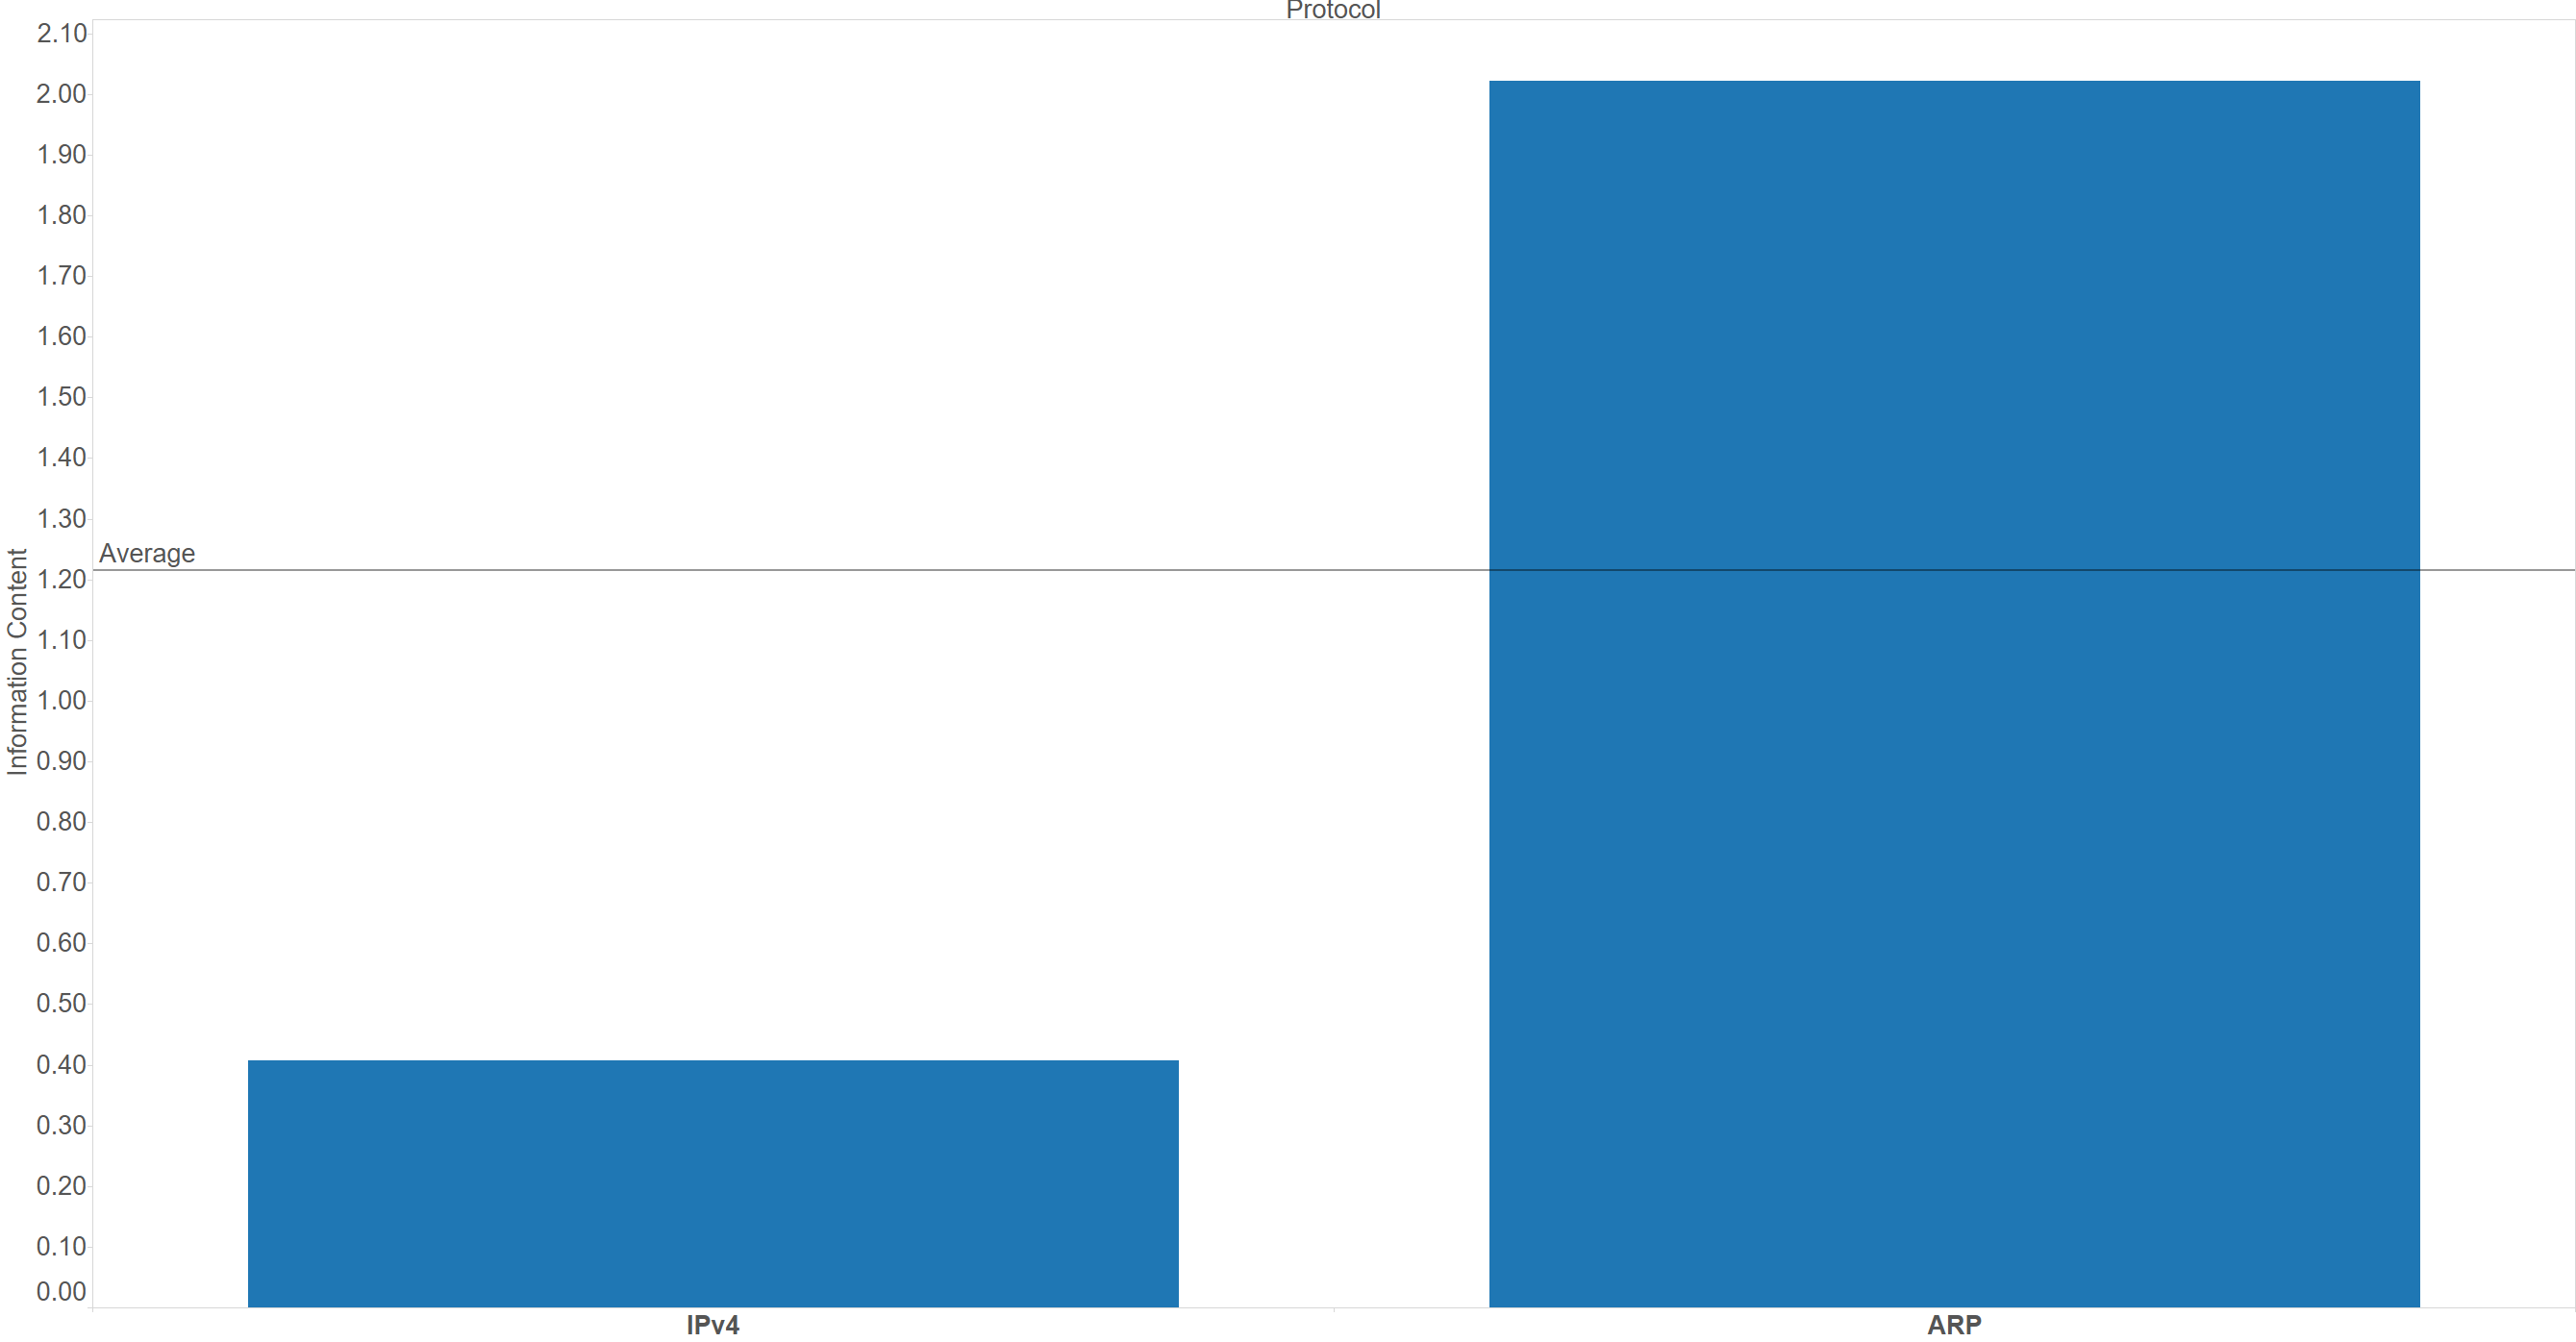
\includegraphics[width=450pt]{captures/McDonalds/20min/Protocol PDF Dashboard.png}
\caption{Cantidad de información de cada símbolo para una fuente que emite los tipos de protocolos encapsulados, con probabilidad para cada símbolo según estimamos a través de la captura de la red}
\end{figure}

Como se puede ver en el gráfico presentado, las incidencias de protocolos en cantidades no consideradas despreciables fueron de ARP e IPv4, tal como habíamos hipotetizado. Además, se cumplió con la ausencia de paquetes de IPv6, situación que no había sucedido en el experimento anterior. Esta situación es la que creemos sería más normal en cualquier tipo de red, ya que la IPv6 aun no está siendo utilizado por los ISPs en Argentina, sería raro encontrar una red que sí tuviera tráfico IPv6 (ya que o sería una red local, o utilizaría algún tipo de túnel al estilo 6-to-4 para conectarse a Internet, pero siempre precisaría de IPv4). 

Observemos que, una vez más, nos encontramos con que tomar el protocolo con menor cantidad de información (o mayor probabilidad) es efectivamente equivalente a tomar el protocolo distinguido, como era de esperarse.

\subsubsection{Distinción de nodos}
\begin{figure}[H]
\centering
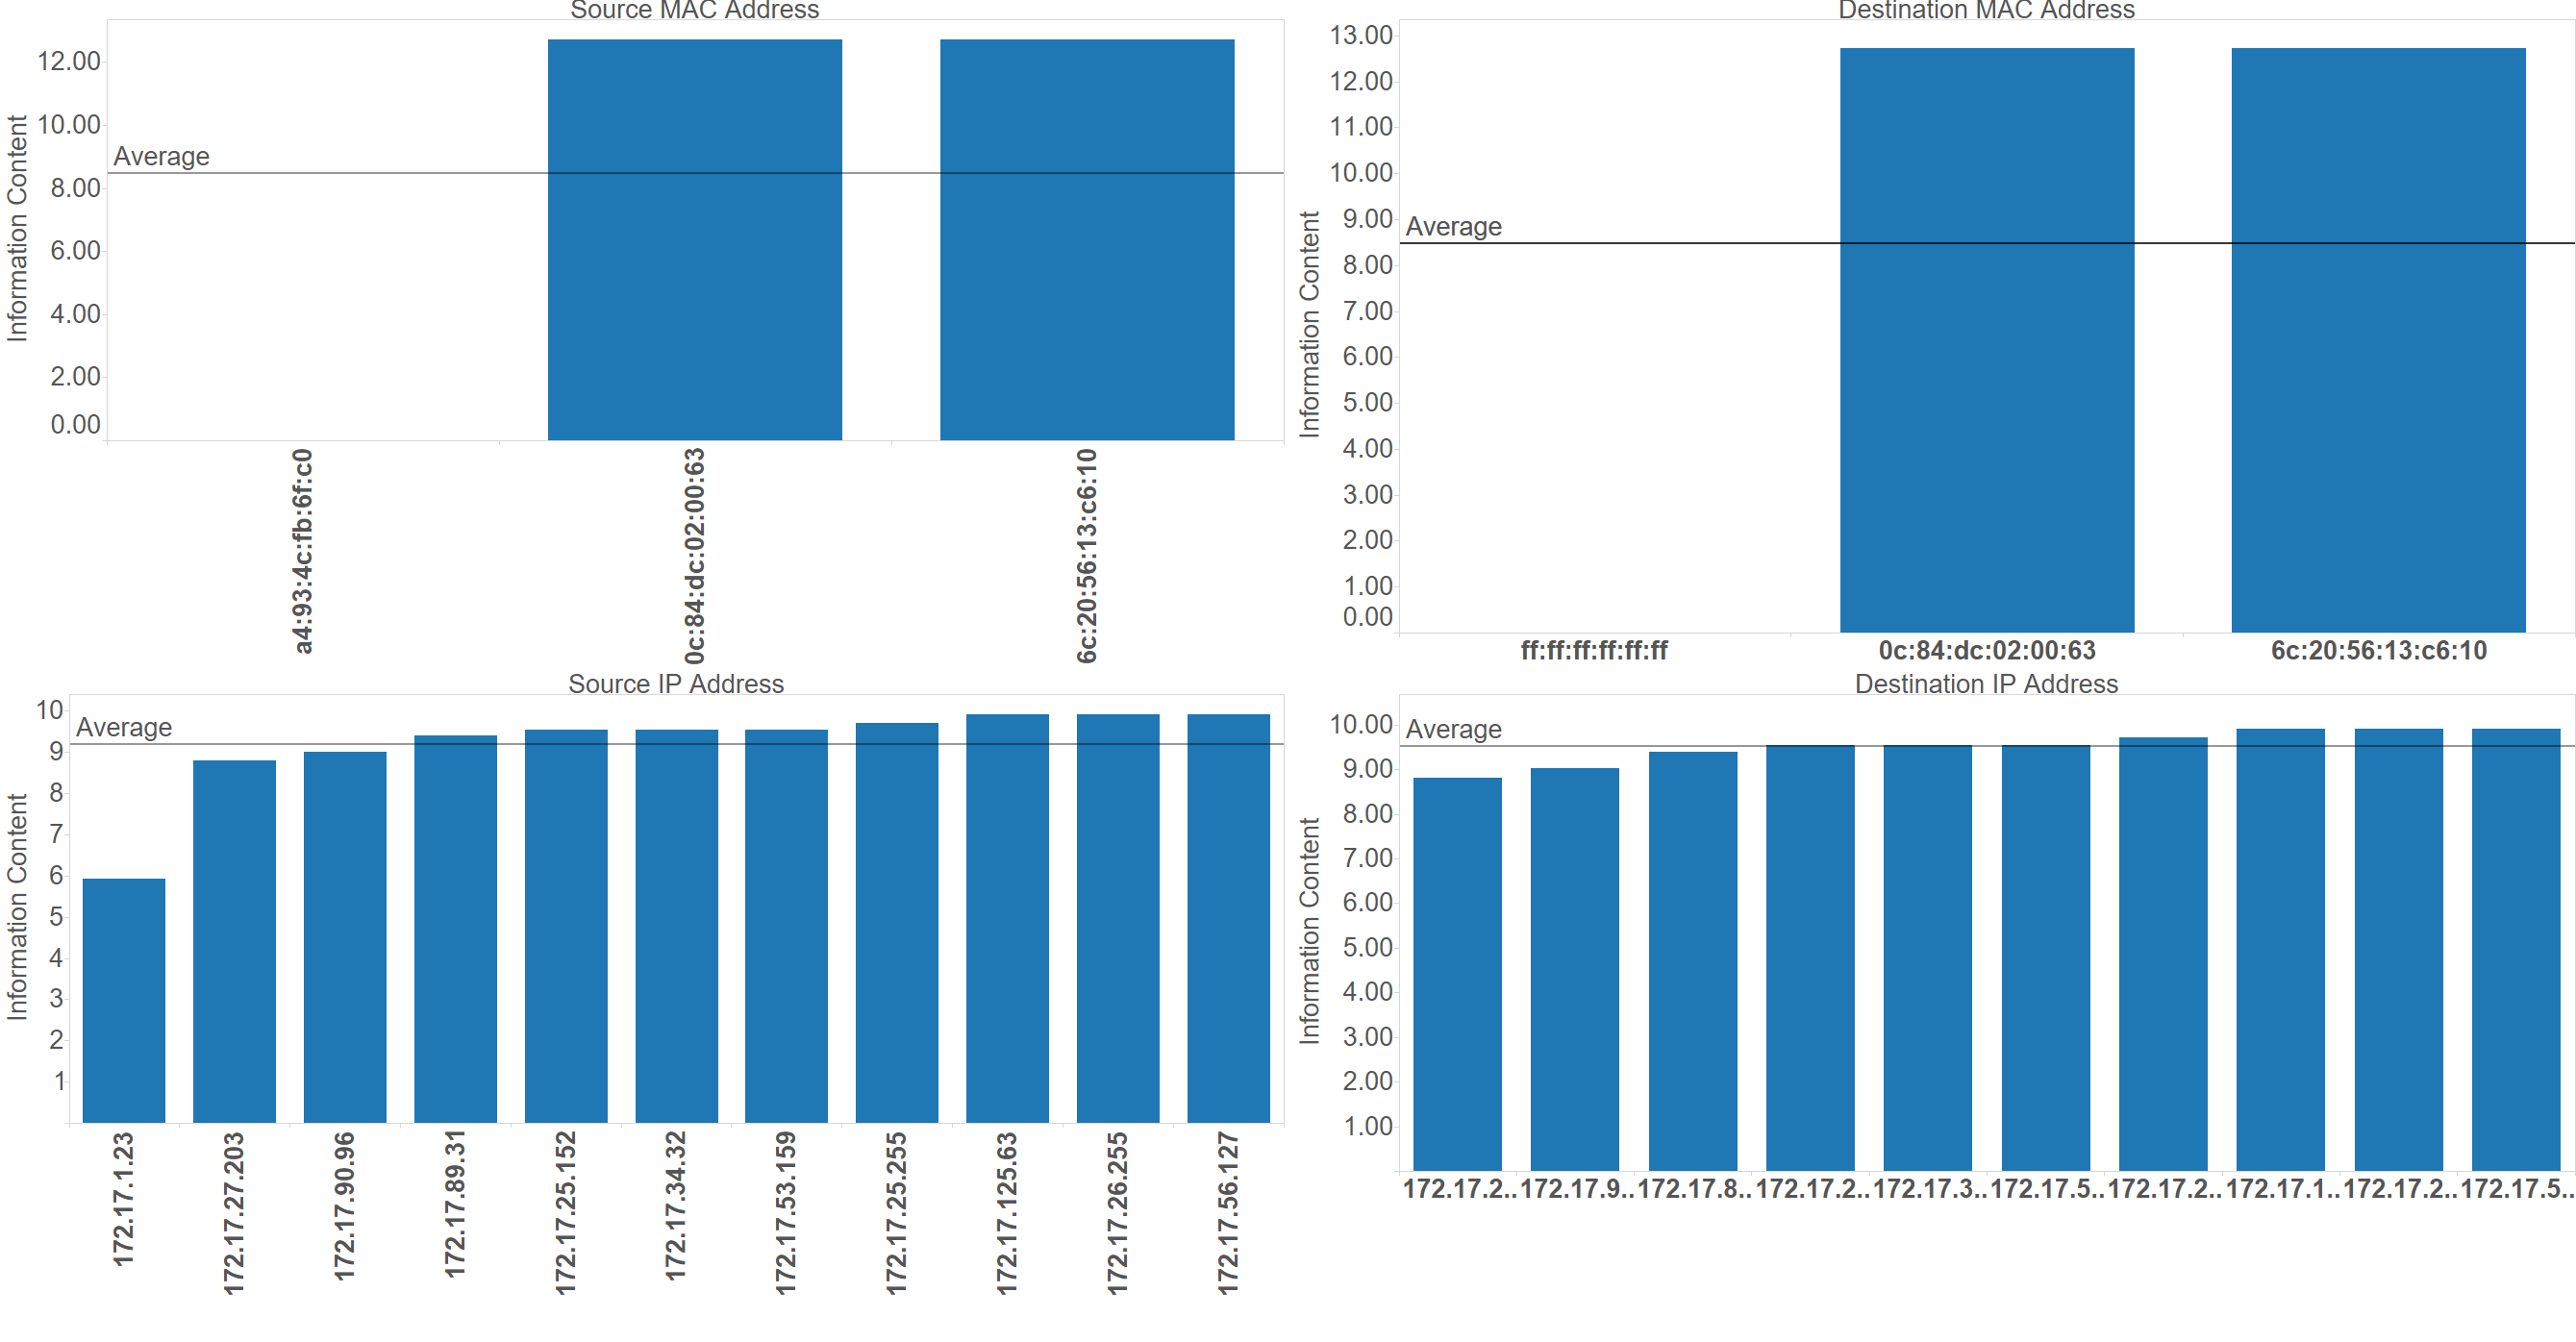
\includegraphics[width=450pt]{captures/McDonalds/20min/PDFs Dashboard.png}
\caption{Para cada gráfico, se muestra en el eje abscisas ponemos los símbolos que consideramos como salida de nuestra fuente de información, y en las ordenadas ponemos la cantidad de información obtenida por la observación del símbolo. Las lineas horizontales muestran el promedio de los valores mostrados, y la entropía de la fuente contemplada, respectivamente.}
\end{figure}

En este caso, la única gran diferencia con respecto de la red anterior es que los valores de la entropía son muy altos en los dos inferiores, y muy bajos en los dos superiores. 

Esto se debe a que en esta red encontramos muchos nodos (IP o Mac Addresses depediendo del gráfico) que no aparecen debido a que su probabilidad es tan baja que fueron filtrados por el corte de probabilidad explicado en la introducción.

Pensamos que la causa de la cantidad de dispositivos con baja probabilidad es que se trataba de una red sin ninguna clave y un dispositivo podía conectarse y desconectarse inmediatamente, porque por ejemplo pertenecía a alguna persona que pasaba por ahí, o simplemente un dispositivo que automáticamente lo hiciese (como sucede con muchos smartphones Android). Observemos que en estos casos, todos esos dispositivos tendrán una cantidad de información relativamente alta en comparación con el router y los otros hosts que puedan estar conectados de forma permanente. El hecho que tengan una cantidad de información tan alta, y sean tantos, genera un bias del promedio hacia los valores más altos, como es de esperar.

En el caso de los gráficos en la parte superior, la entropía es tan baja debido a la gran diferencia en la información que aportan la primer MAC address con respecto a las demás, que además fueron filtradas. El promedio en cambio, es bastante más alto ya que hay más MAC addresses (tanto source como destination) que aportan más información que la primera. En concreto, es la misma situación que describimos en el gráfico anterior, pero con las MAC addresses.

El nodo distinguido, siguiendo el mismo criterio de tomar la Destination IP con menor información en este caso es 172.17.1.23, que efectivamente pudimos corroborar era el router en la red, confirmando que efectivamente el criterio que establecimos parecería funcionar como esperamos.

\newpage
\section{Tercer Experimento: Red Laboral}

\subsection{Presentación}
Para este experimento se analizó una red laboral bastante grande de una empresa de servicios web (MercadoLibre), con una infraestructura de red compleja: hay una única SSID, con múltiples APs distribuidas a lo largo del edificio, y parte de la red es cableada, por lo que tenemos múltiples medios de transporte; además, existen servidores y servicios locales utilizados por muchos usuarios.

En este caso estábamos esperando ver una densidad de paquetes mucho mayor, junto con una mayor presencia de IPv6, y una mayor dificultad del criterio para determinar quién es el router, ya que posiblemente podríamos capturar paquetes de más de un router estando en un mismo lugar.

El tiempo de captura fue de 20 minutos aproximadamente, en el cual se logró capturar alrededor de 160000 paquetes; de los cuales 15000 fueron IPv4, 2700 ARP, 3500 IPv6 y sólo 2 paquetes contenían protocolos desconocidos.

Esta captura presenta una peculiaridad: no se capturaron paquetes de tipo ARP Is At. Utilizando una única computadora (que por otro lado también utilizamos para capturar en las otras redes) y el mismo script, así como intentando utilizar WireShark para descartar bugs, no logramos conseguir este tipo de paquetes.

\subsection{Resultados}

\subsubsection{Protocolos}

Para esta fuente de información, como se dijo previamente, los únicos símbolos presentes fueron 3: IPv4, IPv6 y ARP. Veamos cual es la información de cada símbolo:

\begin{figure}[H]
\centering
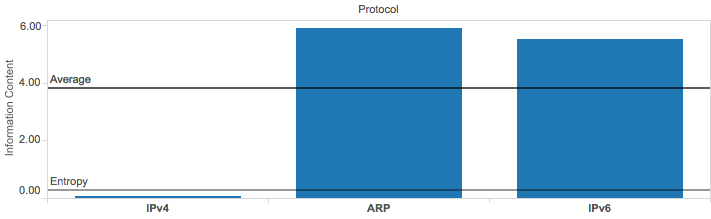
\includegraphics[width=400pt]{captures/MercadoLibre/Protocol PDF Dashboard.png}
\caption{Cantidad de información de cada símbolo para una fuente que emite los tipos de protocolos encapsulados, con probabilidad para cada símbolo según estimamos a través de la captura de la red}
\end{figure}

Se puede ver claramente que IPv4 presenta poca información a la fuente, esto significa que se presenta mucho en esta captura. Además podemos ver que los otros dos protocolos, al mostrar un contenido de información mayor, no parecen haber tenido una incidencia fuerte en nuestra red.

\begin{figure}[H]
\centering
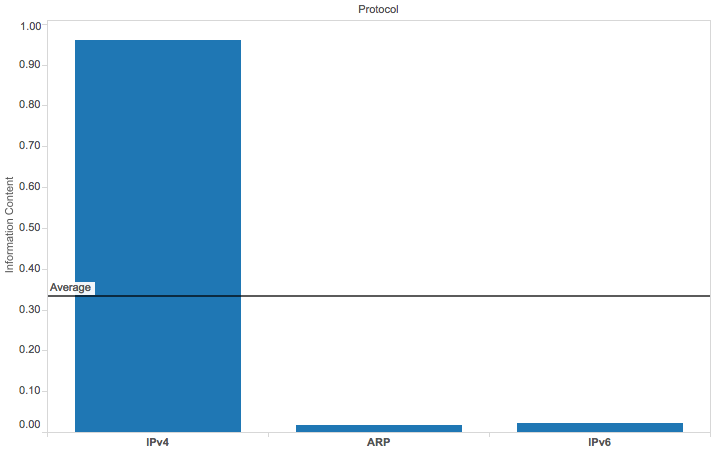
\includegraphics[width=400pt]{captures/MercadoLibre/Protocol PDF Dashboard probability.png}
\caption{Probabilidad de cada protocolo.}
\end{figure}

Estas fueron las probabilidades, para ver los datos mas por el lado de las cantidades.

Es claro que IPv4 fue el protocolo que más se ha manifestado por por una amplia diferencia, lo cual coincide con lo dicho en la presentación de este experimento. 

Es un dato interesante el hecho de que, aunque en poca cantidad, se puede ver un tráfico IPv6, por lo que uno asume que cierta parte de la infraestructura debe haber migrado al nuevo protocolo.

\subsubsection{Nodos ARP}

En este experimento, como se ha dicho antes, no se pude ver ningún trafico capturado de packetes ARP is-at. Esto nos resultó muy extraño, ya que es la base de la capa de enlace.\vspace{1mm}

Conjeturamos que esto podría deberse a una multiplicidad de situaciones:\vspace{1mm}

En primer lugar, en esta red WiFi hay una única SSID pero varios access points, y para nosotros es una incógnita como se maneja el crear una única red local a la que se pueda acceder desde varios puntos de accesos. Por un lado suponemos que debería hacerse un broadcast a todos los AP de todo paquete broadcasteado en cualquiera de ellos, ya que un host va a buscar enviar un paquete a otro host en su subnet utilizando su dirección física y sin necesidad de ser routeado por el AP. Por otro lado, al ser una red tan grande, esto generaría mucho trafico en toda la red local. Lo que terminamos suponiendo es que los paquetes no se broadcastean a todos los APs ya que en ese caso habría una mayor posibilidad de ver ARP Is At, pero la falta de conocimiento no nos permite llegar a una conclusión al respecto.\vspace{1mm}

En segundo lugar, es posible que el uso de múltiples medios de transmisión sea el causante de un problema: la resolución de direcciones fuese para hosts conectados únicamente por cable, recibiríamos el broadcast del Whois pero jamás recibiríamos la respuesta, ya que esta sería forwardeada a través de los cables. Por otro lado, una situación similar podría darse en una conexión donde una parte es por cable y otra por Wi-Fi, ya que simplemente podríamos o no llegar a capturar el paquete por algún tipo de ruido en el medio, o simplemente estar lejos del nodo Wi-Fi receptor.\vspace{1mm}

Esta última situación puede suceder inclusive entre dos nodos conectados por Wi-Fi si consideramos que podrían tener un radio lo suficientemente chico como para que cada uno alcance a comunicarse con el router pero no alcance a capturar el tráfico hacia el otro nodo.\vspace{1mm}

Dejando esta situación atrás (y ya que no podemos tampoco determinar cuál es la realidad, al no tener acceso a la infraestructura), y como en los experimentos anteriores, tomaremos como símbolo de la fuente de información a varios campos del paquete ARP por separado: MAC source, MAC destination, IP source y IP destination.

\par Veamos qué capturamos desde el punto de vista de la cantidad de información:

\begin{figure}[H]
\centering
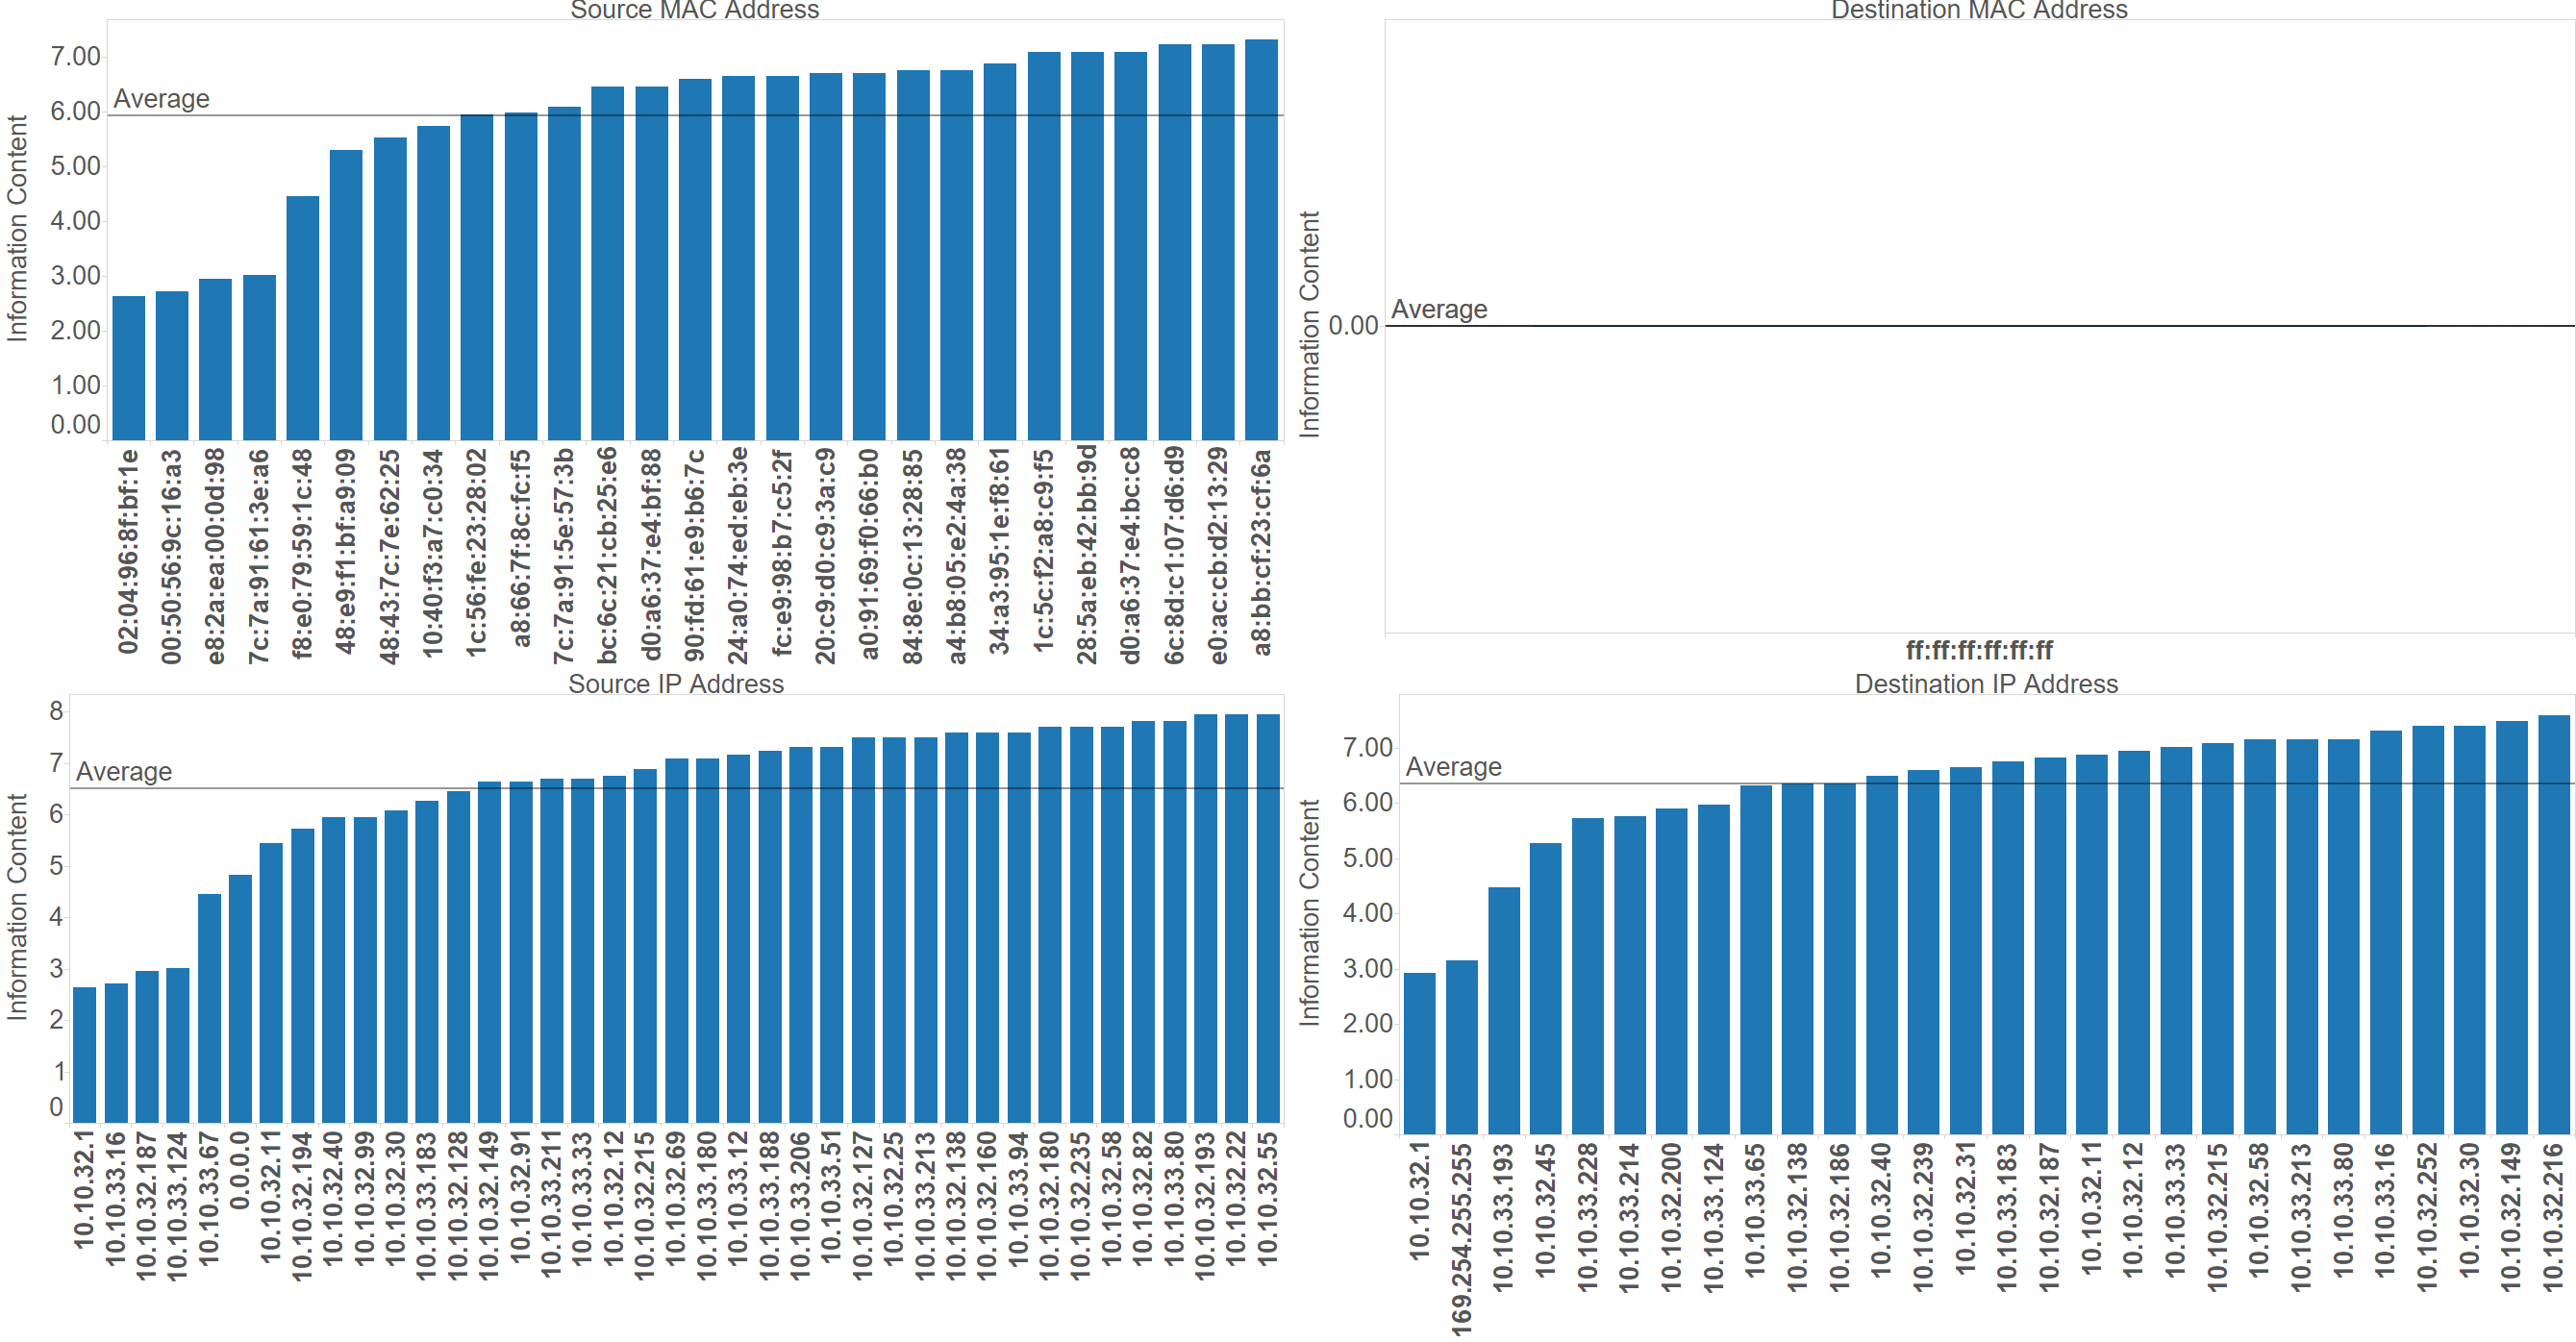
\includegraphics[width=420pt]{captures/MercadoLibre/PDFs Dashboard.png}
\caption{Información de cada símbolo, para cada fuente de información.}
\end{figure}

Vayamos uno por uno:\vspace{2mm}

Tomando a cada MAC source de los paquetes ARP como símbolos podemos ver que, los que dan menos información son principalmente los primeros 4: \textbf{02:04:96:8f:bf:1e}, \textbf{00:50:56:9c:16:a3}, \textbf{e8:2a:ea:00:0d:98} y \textbf{7c:7a:91:61:3e:a6},  los cuales otorgan aproximadamente una misma cantidad de información, por lo tanto llegamos a la conclusión de que estos cuatro MAC pertenecen a nodos claves de la red.\vspace{1mm}

Tomando a cada IP source como simbolo llegamos a algo parecido, hay 4 IP que otorgan una cantidad de información aproximada y son los que otorgan menos información: \textbf{10.10.32.1}, \textbf{10.10.33.16}, \textbf{10.10.32.187} y \textbf{10.10.33.124}

Chequeando la tabla ARP cacheada por mi host en esta red en el momento de captura se llego a que efectivamente estas 4 IPs pertenecen a esas 4 MACs en respectivamente.\vspace{1mm}

Tomando a la MAC destino como simbolo no llegamos a ninguna conclusión, porque, como ya dijimos, no capturamos ningun paquete ARP is-at, por lo tanto todos los paquetes considerados son ARP who-is, un host al enviar un paquete ARP who-is siempre hace Broadcast para que todos los host dentro de la misma red local. Esto quiere decir que el unico simbolo capturado va a ser el de MAC de Broadcast: \textbf{ff:ff:ff:ff:ff:ff}.\vspace{1mm}

Tomando a la IP de destino como símbolo podemos ver 2 IPs que otorgan una misma cantidad de información aproximadamente, siendo esta la mínima.
Estas dos IPs son: \textbf{10.10.32.1} y \textbf{169.254.255.255}
Según analizamos, la IP \textbf{169.254.255.255} pertenece a un rango de IPs reservadas que se asigna un host cuando no se le asigna ninguna IP especifica (el DHCP todavía no le asigno una IP o no se la va a asignar). Por lo tanto no nos sirve de mucho, de hecho se puede llegar a la conclusión de que la fuente de información formada de esta forma nos resalta ruido mas que información. 
Por otro lado vemos que la IP  \textbf{10.10.32.1} se repitió también en el anterior gráfico como destacado, lo cual no hace estar mas seguros que esa IP pertenece a un nodo importante en la red.\vspace{1mm}

Teniendo en cuenta este análisis converjo a creer que la primera y la segunda fuente de información (tomando a los símbolos como la source MAC y la source IP respectivamente) son las mejores a la hora de averiguar cuales son los nodos importantes de una red. Ya que efectivamente, el nodo con la IP \textbf{10.10.32.1} era el Default Gateway de la red local.
Al mismo tiempo, el nodo con la IP \textbf{10.10.33.16} era un nodo por le que pasa trafico de forma interna para no tener que acceder a partes de la aplicación a través de internet.

Sin saber esto por tener acceso al administrador de red, gracias a la herramienta de análisis que elaboramos, uno puede llegar a la concluir que estos nodos cumplen un rol importante en la red, que pasa mucho trafico a través de ellos, y esto significa que seria un buen punto de ataque para ataques de Denegación de Servicios o para simplemente capturar datos en cantidad y buscar informacion sensible.

\newpage

\section{Cuarto Experimento: Red Controlada}

\subsection{Características y condiciones de la red}

Dado que ya analizamos tres redes con una cantidad importante de nodos y tráfico, decidimos en este experimento tratar con una red casera debido a que tenemos más control sobre la misma y podemos verificar las hipótesis de forma concreta por ser más fáciles de comprender. Se trata de una red Wi-Fi compuesta por siete dispositivos (entre ellos tablets, celulares y computadoras).

Además, para mejorar las probabilidades de tener un tráfico de paquetes ARP considerable, reiniciamos el router antes de comenzar a capturar el tráfico con el objetivo de vaciar la caché ARP del router.

Como se trata de una red de pequeñas dimensiones, para poder hacer una captura que realmente nos brinde información valiosa necesitamos estar capturando el tráfico un tiempo mayor que en los casos anteriores. En las redes anteriores si hacíamos capturas de unos pocos segundos ya teníamos muchísimos datos por las dimensiones de las redes y por eso los tiempos de captura eran relativamente cortos. Es por eso que en este caso decidimos capturar el tráfico durante una hora.

\subsection{Resultados}

\subsubsection{Grafo de tráfico ARP}
\begin{figure}[H]
    \centering
    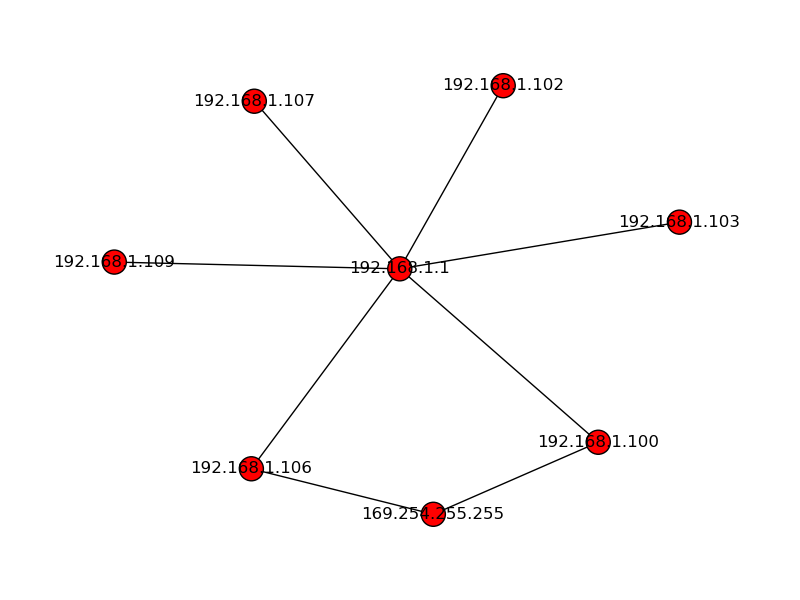
\includegraphics[width=0.70\textwidth]{../captures/CasaGerman/conn_ip.png}
    \caption{Tráfico de paquetes ARP en la red, distinguiendo nodos por IP.}
    \label{fig:mesh1}
\end{figure}

El gráfico anterior nos permite tener un panorama general de los nodos de la red según el envío de paquetes ARP. Lo primero que puede parecer extraño al observar este gráfico es que aparece una IP un tanto extraña (169.254.255.255) en comparación con las demás. Investigamos un poco sobre este tema y resulta que esta IP es asignada a un dispositivo de manera automática cuando no encuentra otra. Esto es muy común que suceda en sistemas Windows aunque también pasa en dispositivos Mac y se da cuando existe algún problema para asignar una IP al dispositivo.
\par Otra cosa que podemos ver es que el grafo tiene una forma de estrella centrada en un nodo cuya IP es 192.168.1.1, tiene sentido pensar que este nodo es el router ya que es el que se comunica mediante el protocolo ARP con todos los demás nodos (excepto el que tiene una IP distinta por motivos que ya explicamos antes). Debido a que esta es una red conocida por nosotros, pudimos efectivamente corroborar esto (comando route -n de Ubuntu) y era verdad, el nodo cuya IP es 192.168.1.1 corresponde al router.

\begin{figure}[H]
    \centering
    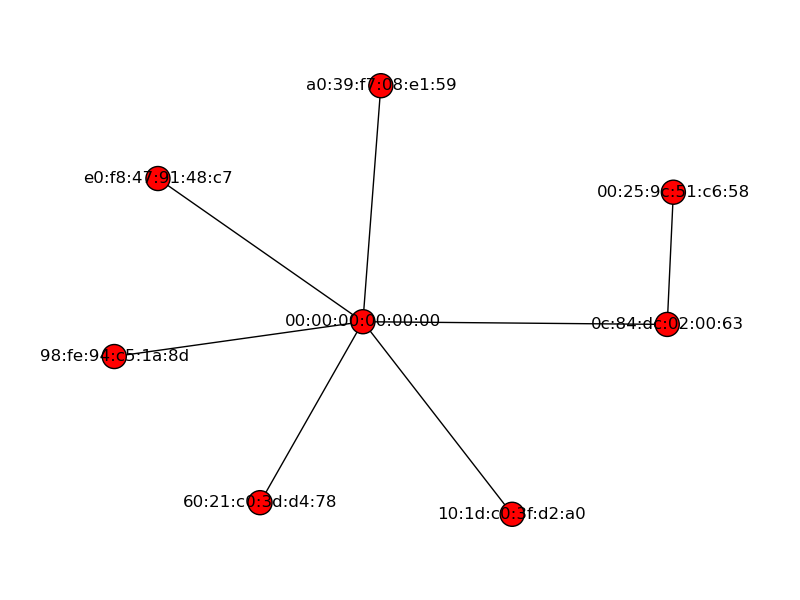
\includegraphics[width=0.70\textwidth]{../captures/CasaGerman/conn_mac.png}
    \caption{Tráfico de paquetes ARP en la red, distinguiendo nodos por Mac Address.}
    \label{fig:mesh1}
\end{figure}

Este gráfico es similar al anterior en el sentido de que nos revela el tráfico de paquetes ARP pero nos permite diferenciar a los nodos segun sus Mac Addresses.

\subsubsection{Distinción de protocolos}
\begin{figure}[H]
    \centering
    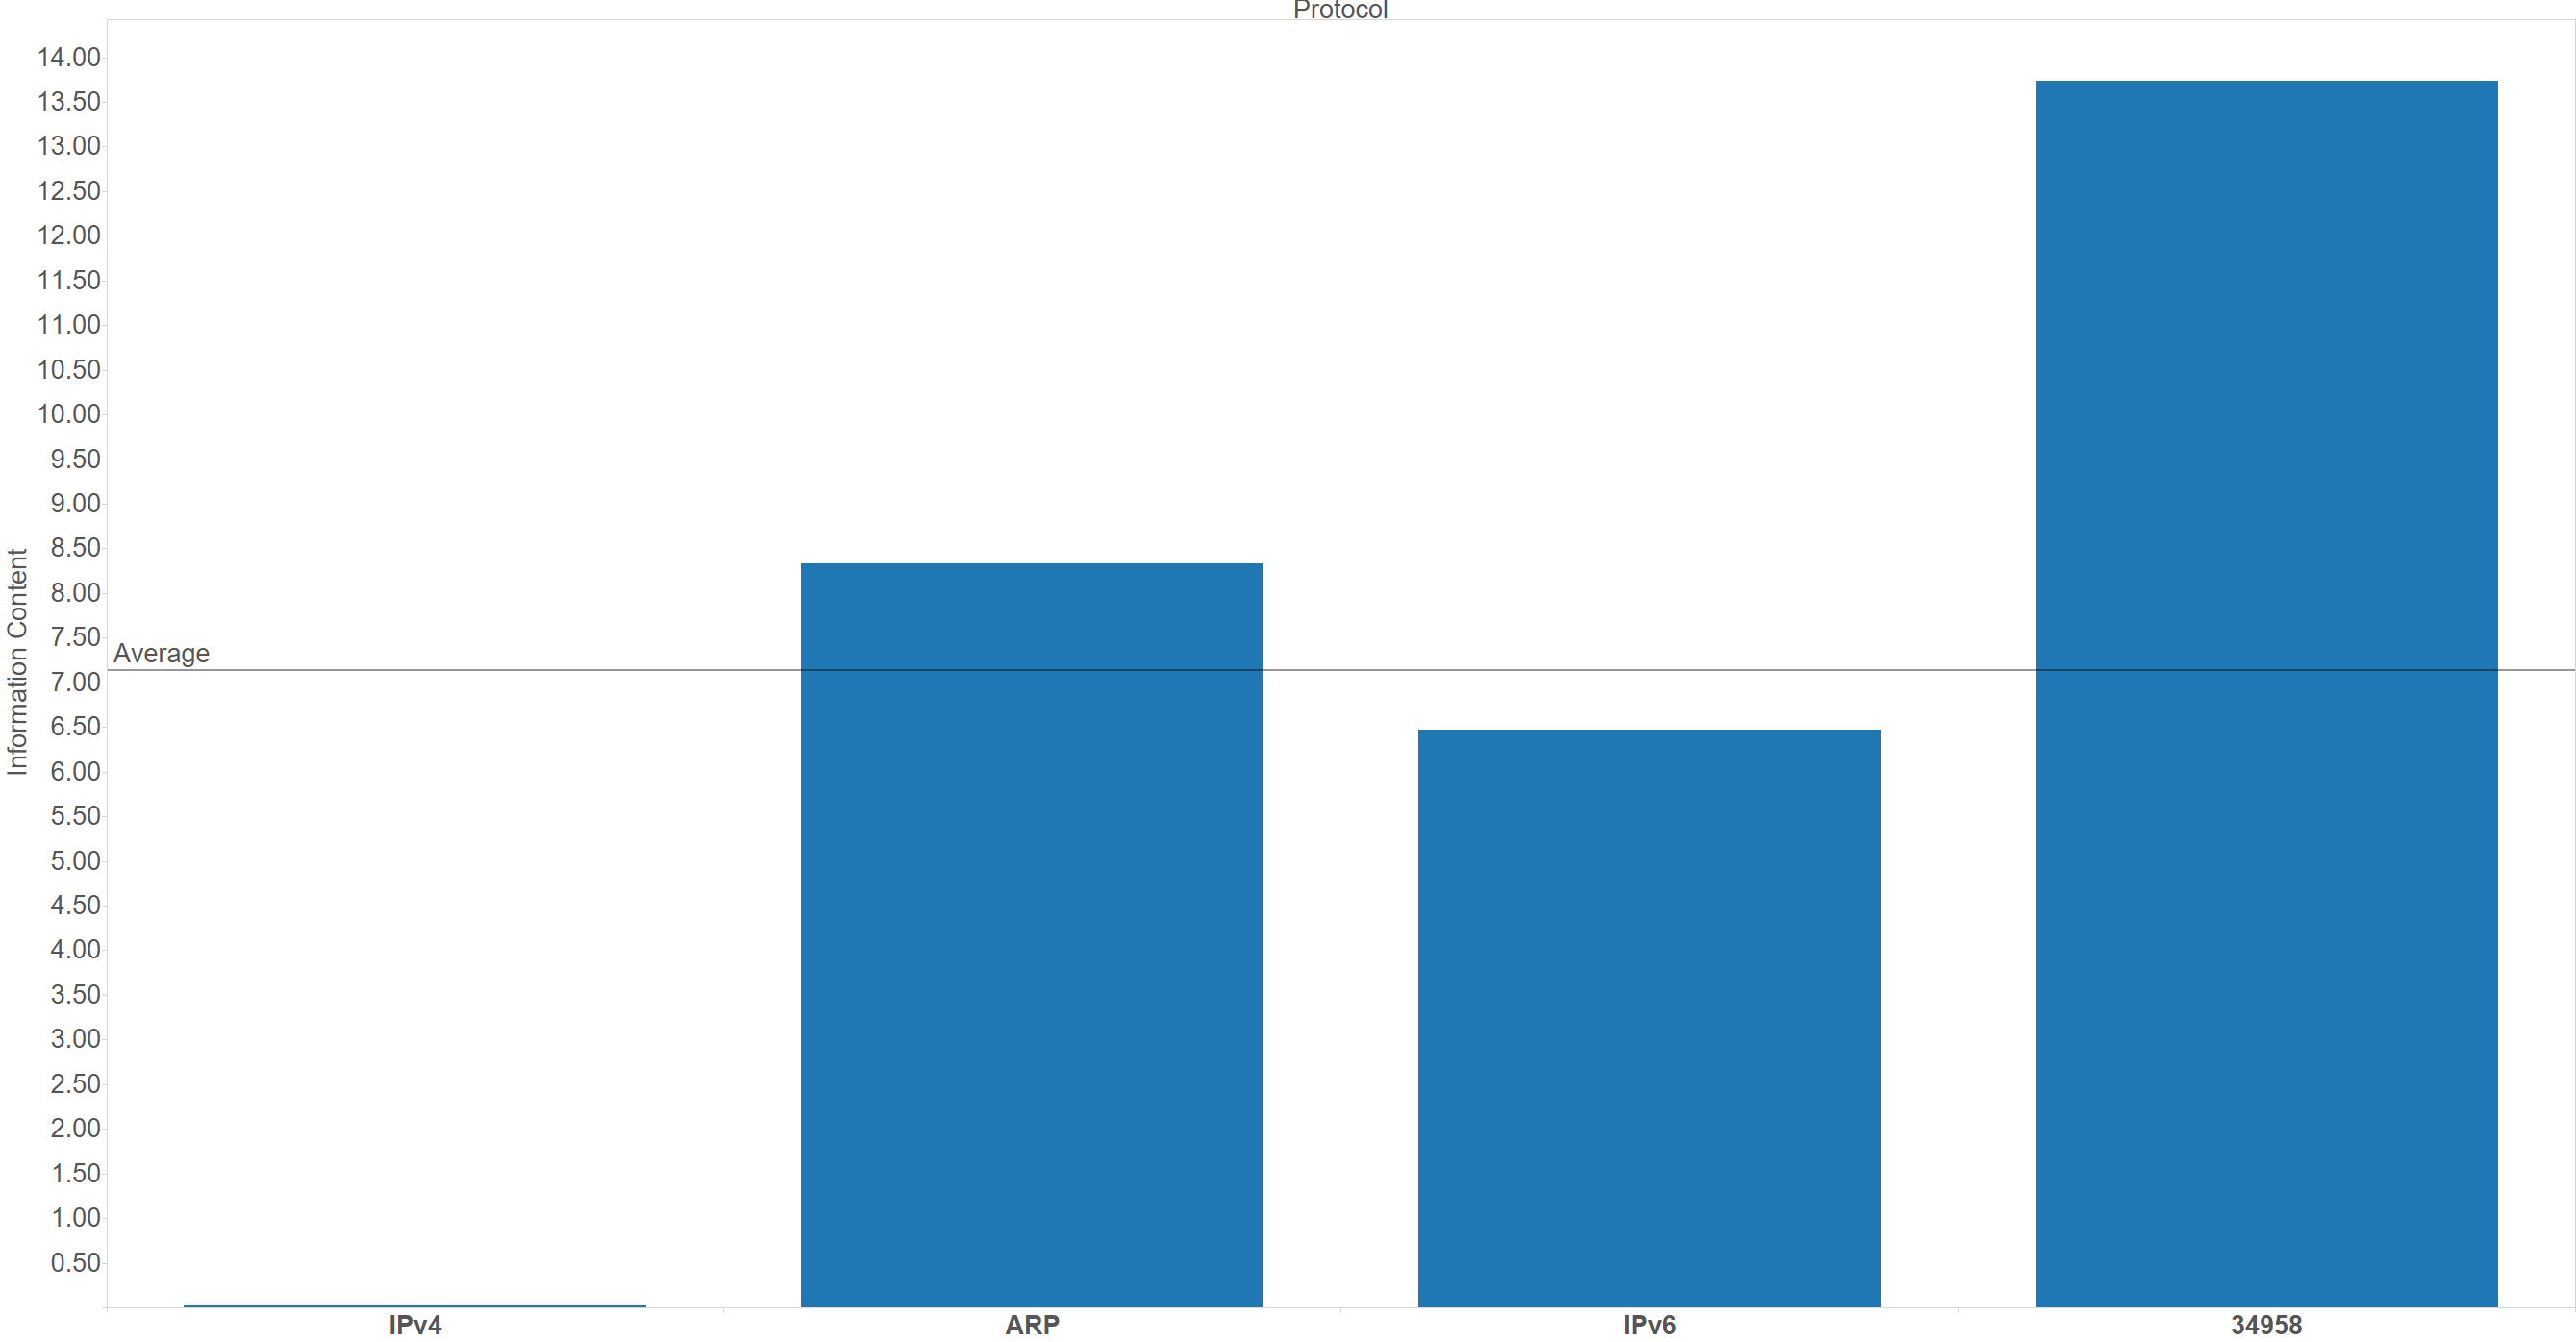
\includegraphics[width=1\textwidth]{../captures/CasaGerman/Protocol PDF Dashboard.png}
    \caption{Este gráfico nos muestra la cantidad de información que provee cada protocolo a la fuente (donde los símbolos son los protocolos), información promedio y entropía.}
    \label{fig:mesh1}
\end{figure}

Si observamos la línea que representa la entropía, vemos que se trata de un valor muy bajo, indicando que se trata de una fuente predecible en cuanto a los símbolos que emite.

En cuanto a los símbolos en sí, vemos que la información proveída por IPv4 es muy pequeña mientras que la del protocolo 34958 es muy alta y las correspondientes a ARP e IPv6 son alrededor de la mitad de 34958. El protocolo distinguido es claramente IPv4 ya que es el que menos información tiene y por lo tanto el más utilizado. Los otros protocolos tienen información bastante más elevada, esto se debe a que al ser una red casera el tráfico de paquetes ARP (por ejemplo) es bastante más reducido ya que la cantidad de dispositivos es reducida y es más fácil y rápido para el router llenar la caché que vincula IP Addresses con Mac Addresses.

\subsubsection{Distinción de nodos}
\begin{figure}[H]
    \centering
    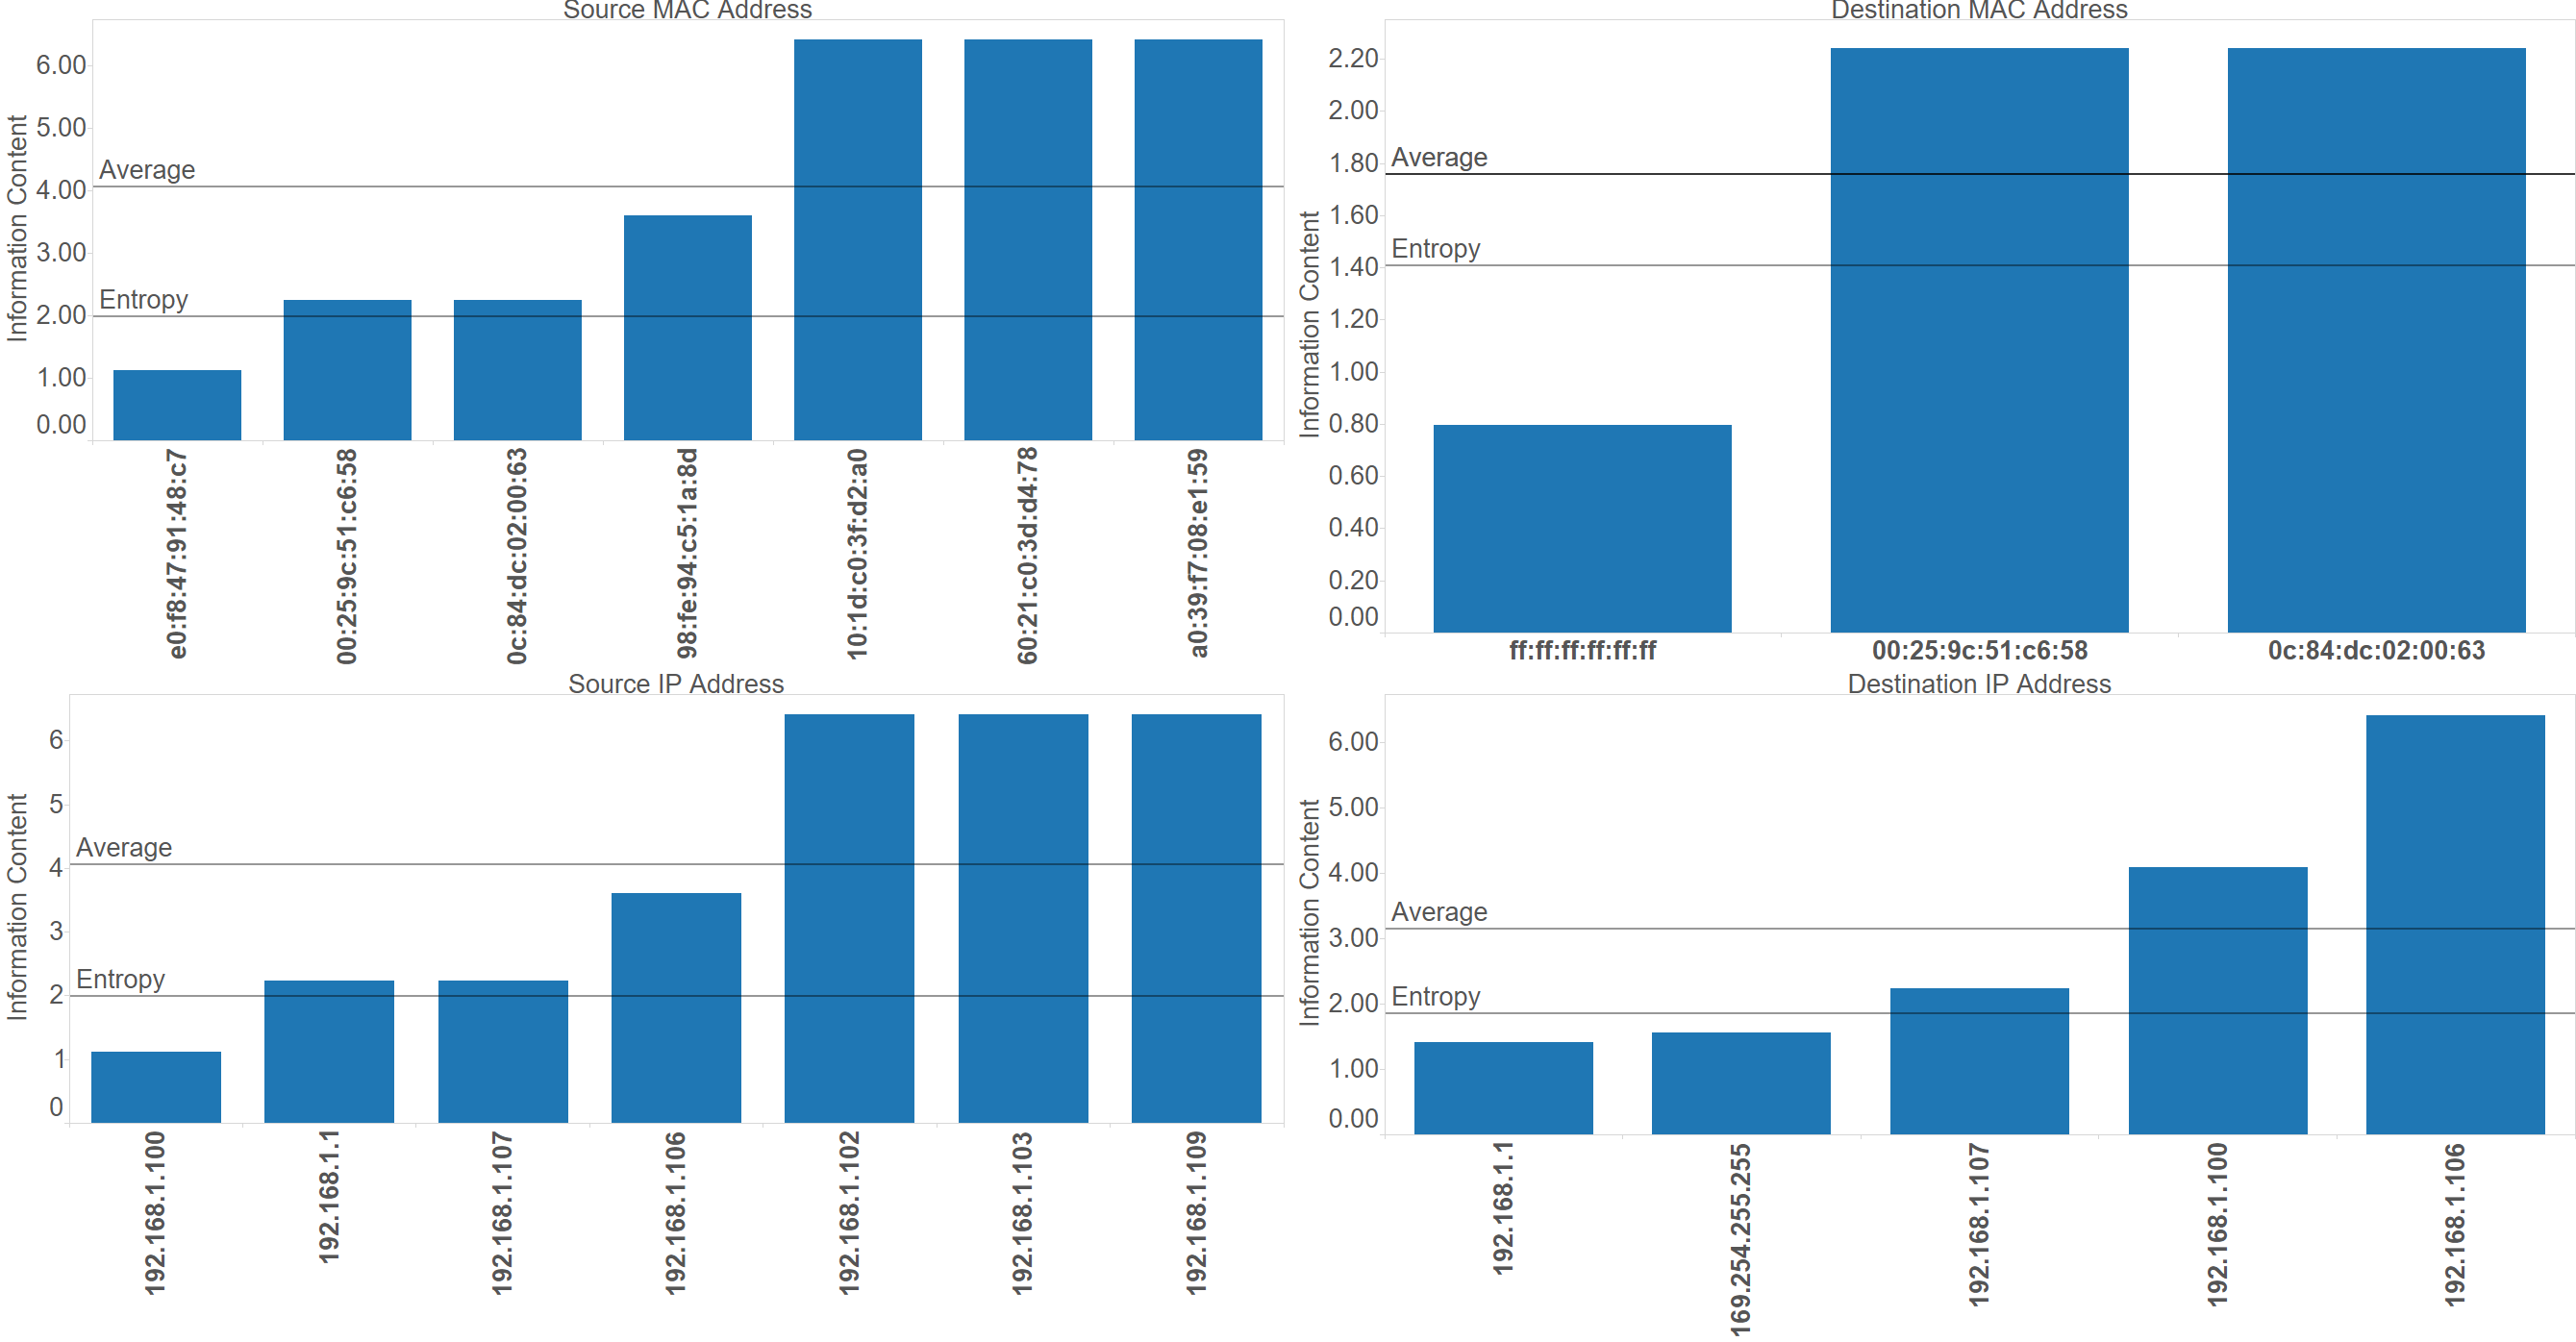
\includegraphics[width=1\textwidth]{../captures/CasaGerman/PDFs Dashboard.png}
    \caption{Al capturar paquetes ARP y quedarnos con las direcciones Mac de source como símbolos de la fuente obtenemos el gráfico de la esquina superior izquierda que nos muestra la información de cada nodo (visto como Mac Address), si nos quedamos con las Mac de destino de los paquetes obtenemos el de la derecha que nos muestra la información de cada nodo. Análogamente tenemos los gráficos de abajo que utilizan direcciones IP.}
    \label{fig:mesh1}
\end{figure}

Para poder elegir el nodo distinguido (podría ser más de uno) vamos a utilizar el gráfico de Destination IP Address y tomar la IP de destino con menor cantidad de información (respetando así el criterio fijado al principio). En este caso dicha IP es 192.168.1.1 que es la correspondiente al router como habíamos aclarado antes. Esto tiene mucho sentido ya que el mayor tráfico que pasa por la red involucra al router y se corresponde con el primer gráfico que mostramos en este experimento (el grafo con forma de estrella).

\subsubsection{Relación IP Address - MAC Adrress}
\begin{figure}[H]
    \centering
    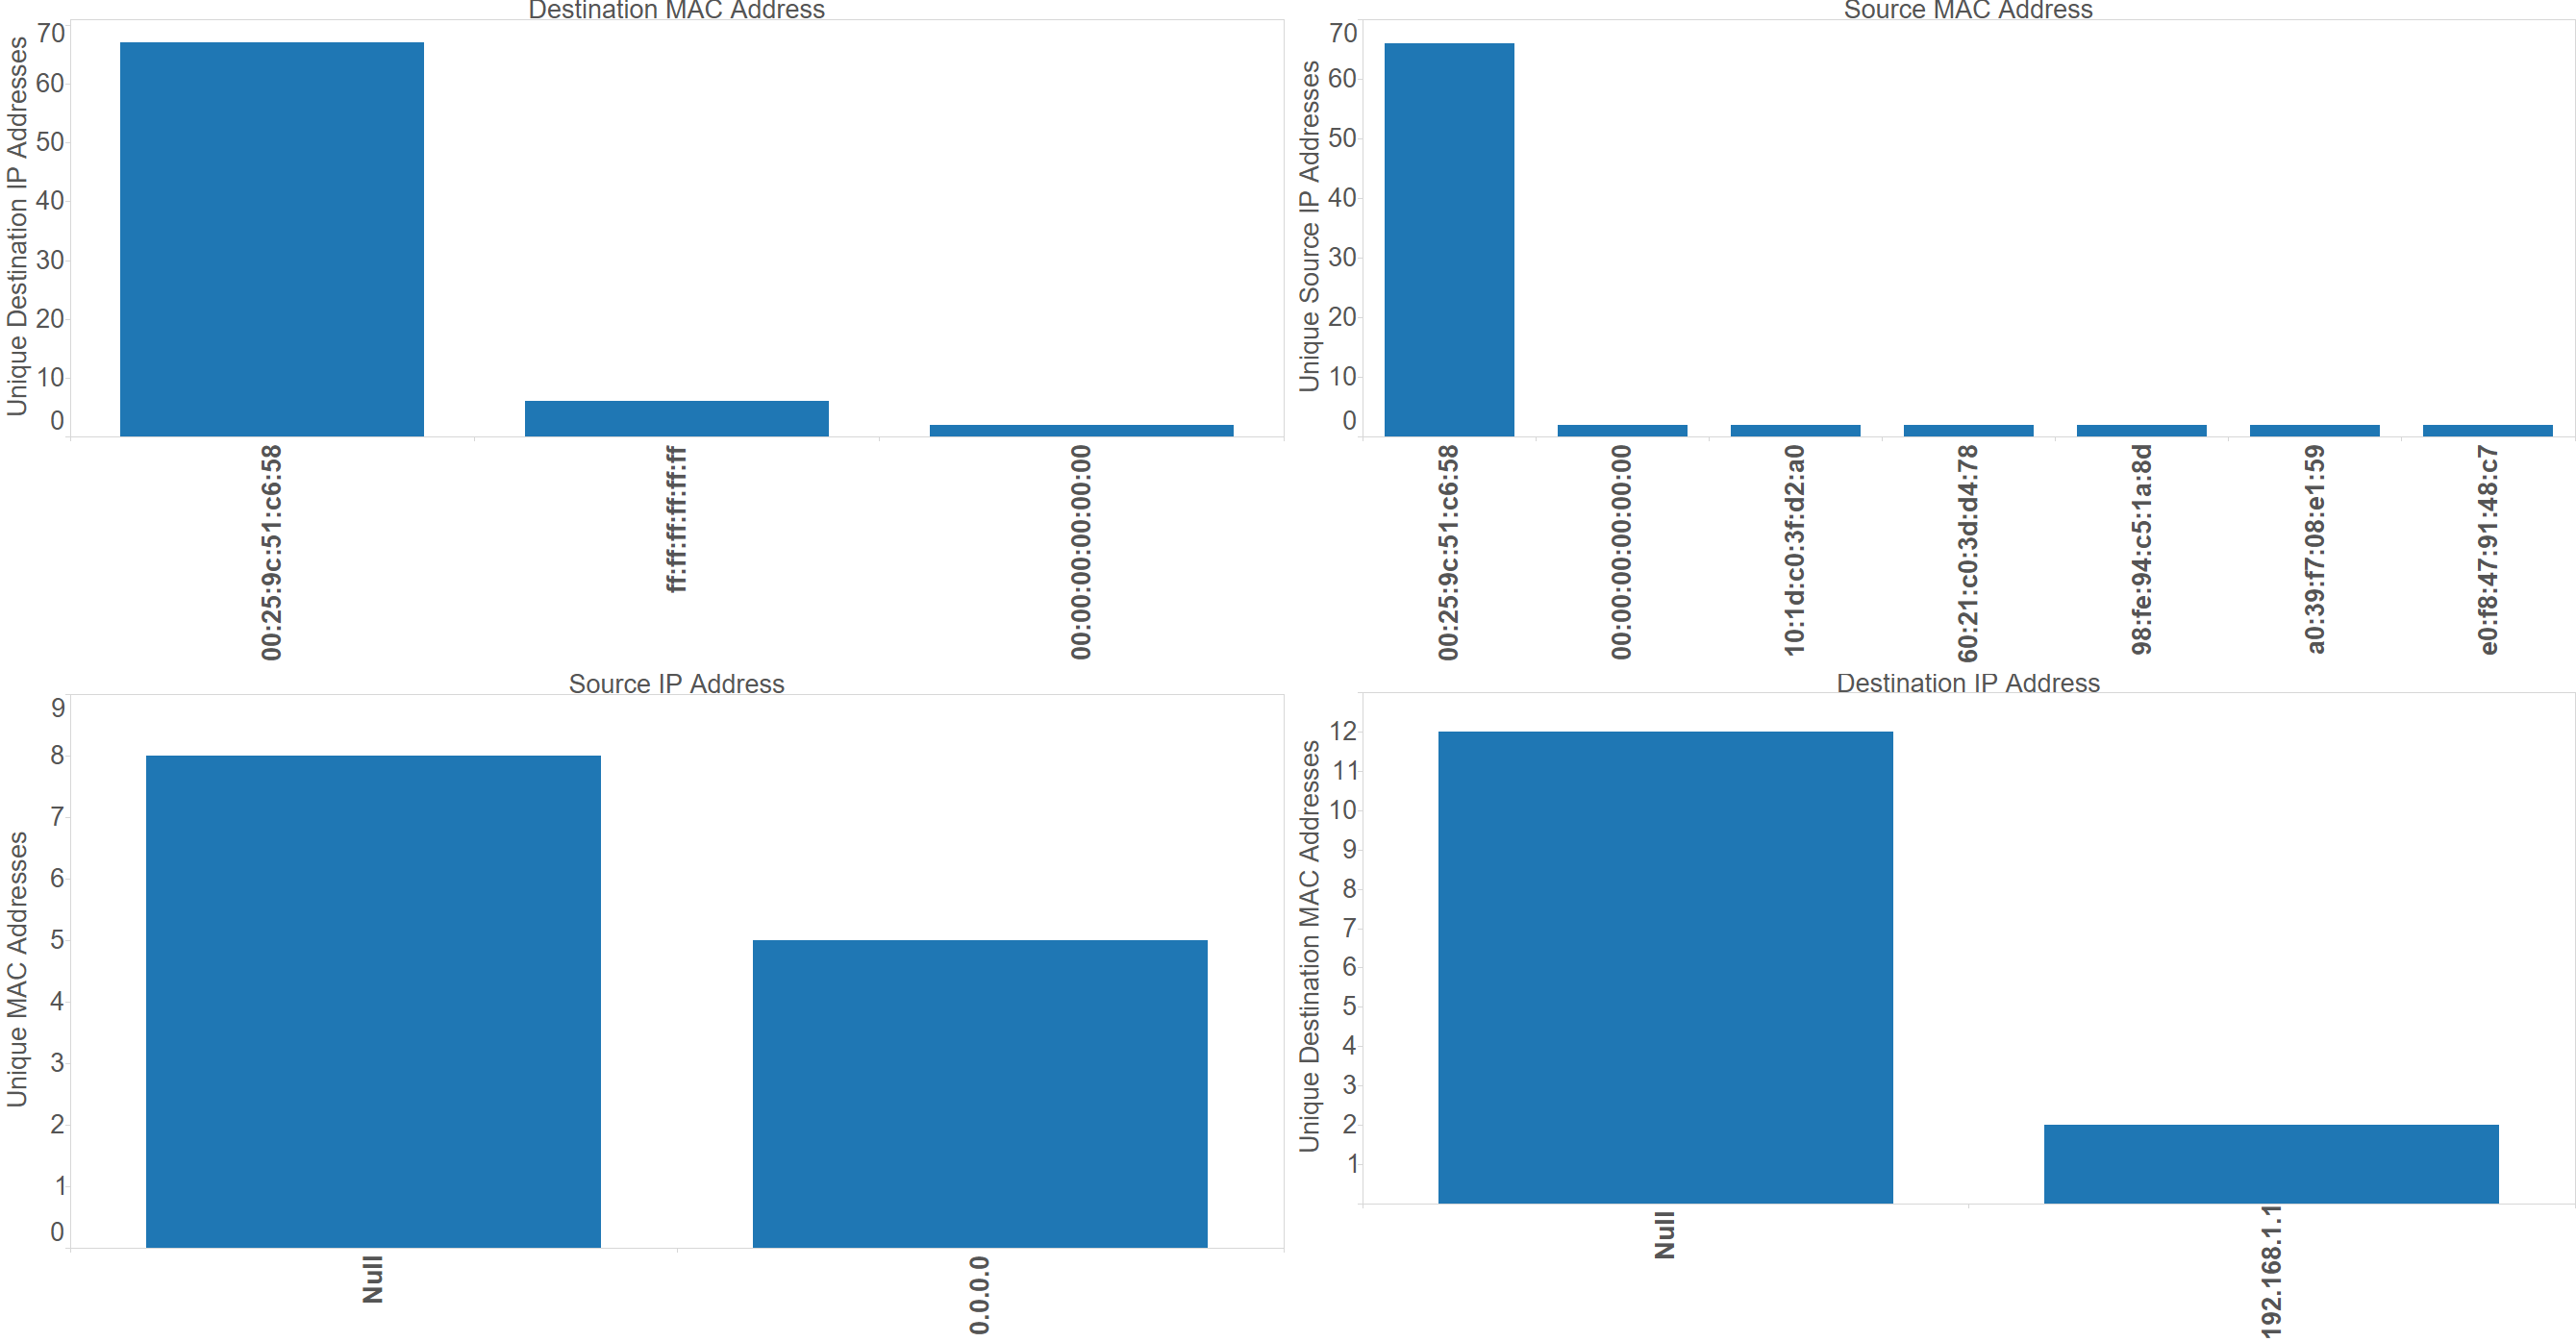
\includegraphics[width=1\textwidth]{../captures/CasaGerman/IP vs MAC Correspondence.png}
    \caption{Estos cuatro gráficos nos dan información sobre la relación entre las IP y Mac Addresses.}
    \label{fig:mesh1}
\end{figure}

El gráfico que se encuentra en la esquina superior izquierda nos muestra la cantidad de IP's distintas a las cuales fueron dirigidos paquetes provenientes de las Mac Addresses mostradas. El de la derecha por el contrario, nos muestra la cantidad de paquetes de distintas IP's que tienen por destino una misma Mac Address. La Mac Address que más recibe y más envía es 00:25:9c:51:c6:58 y casualmente corresponde al router (corroborado con el comando arp -n de Ubuntu). La dirección de broadcast (ff:ff:ff:ff:ff:ff) también se hace notar un poco en el primer gráfico. Esto último es razonable ya que es la que se encarga de enviar paquetes a todos los dispositivos de la red y por lo tanto va a tener tantas IP's distintas de destino como dispositivos conectados a la red con una IP asignada válida existan.

En cuanto a los gráficos de abajo, el de la izquierda nos dice, dada una IP, cuantas Mac Addresses distintas tuvieron dicha IP como fuente en los paquetes capturados. El gráfico de la derecha nos dice la cantidad de Mac Addresses distintas que aparecieron en paquetes enviados a una misma IP. Sin embargo, estos dos gráficos no nos dan mucha información debido a que por motivos que tienen que ver con la implementación de Scapy, sucede que para todos los paquetes cuyos protocolos son IPv6 o cualquier otro que no mencionamos en este informe, no es posible conseguir la dirección de IP. Las IP ``válidas'' que aparecen son solo dos, una es el router (192.168.1.1) y la otra es 0.0.0.0 que se utiliza cuando no se tiene asignado todavía una IP (por eso válidas entre comillas).

\section{Conclusiones}

Encontramos que las redes analizadas tienden a acentuar ciertos hosts como los que más tráfico generan (y reciben); como habíamos conjeturado en la introducción, estos suelen ser los gateways que permiten conectarse a Internet. No es una sorpresa esto, ya que en general, y en particular en los tipos redes Wi-Fi que analizamos (excluyendo el caso de MercadoLibre, que brilla por ser una red bastante más compleja que en los otros casos), las redes Wi-Fi no suelen ser utilizadas para conectar dispositivos dentro de la misma red, sino para proveer acceso a Internet.

Encontramos que cada red presentó características únicas con respecto a las otras: la de MercadoLibre nos mostró una situación donde en realidad hay un único SSID pero múltiples AP a la red local, junto con las complicaciones que esto trae, mientras que las redes públicas abiertas nos mostraron una gran cantidad de nodos y un bias de la entropía hacia valores más altos debido a la gran cantidad de hosts conectados de forma efímera; y también observamos el hermoso funcionamiento de una red pequeña donde casi que parecería que los protocolos no fallan.

Además, encontramos el fenómeno mencionado anteriormente donde logramos capturar cantidades de ARP Whois mucho mayores a ARP IsAt, lo que nos permitió formular las conjeturas sobre los posibles problemas para capturar ARP en redes que cubren amplias distancias, utilizan medios mixtos, o simplemente utilizan Wi-Fi.

El hecho de hacer un experimento sobre una red controlada, como punto de comparación con las otras 3 redes (una semi-controlada, la de MercadoLibre, y las otras dos públicas y abiertas), nos permitió poder corroborar algunas de las hipótesis y forzar ciertas condiciones sobre la misma antes de comenzar la captura que no hubiera sido posible hacerlo con redes no controladas como las anteriores.

En redes caseras como esta vemos que el router tiene una incidencia importante y el tráfico de paquetes suele ser reducido. En particular la cantidad de paquetes ARP fue muy reducida (incluso reseteando el router antes de comenzar las capturas) y los de IPv4 predominaron. Esto puede ser debido a varias razones:

\begin{itemize}
\item Los distintos nodos conectados suelen guardar las direcciones MAC ya conocidas en una caché, en consecuencia no suele ser necesario recurrir a los protocolos ARP de manera frecuente.

\item Por otro lado, también ocurre que no suele haber mucho movimiento en los nodos en una red Wi-Fi controlada y no pública (refiriéndonos a movimiento como ingreso de nodos nuevos de manera seguida). Esto contrasta de manera clara con los experimentos de redes públicas, en los que podemos suponer que hay una clara relación entre el movimiento de la gente por el espacio que provee dicha red y los dispositivos que se conectan a la red provista.
\end{itemize}

En términos del criterio elegido, el mismo funcionó de forma infalible en todas las redes que probamos, con el detalle de ser difícil de generalizar a más de un router (simplemente porque la entropía puede ser un valor arbitrariamente alto, y entonces no es fácil tomar un corte). Sin embargo, tomar siempre el Destination IP Address con menor cantidad de información funcionó consistentemente para encontrar un router dentro de la red. Cabe destacar, sin embargo, que no pudimos capturar paquetes en una red con un servicio muy centralizado como para ver qué pasa (y esto es un punto donde podrían realizarse experimentos a futuro).

Como una posible idea de experimentación, pensamos que sería un criterio casi infalible utilizar el Destination MAC Address de los paquetes IPv4 junto con un conocimiento de la(s) subnet(s) de la red local, ya que de esta forma podríamos saber explícitamente cuándo un paquete debe ser enviado hacia la Internet, y por ende la Destination MAC Address sería la del router, y la Destination IP Address una IP fuera de la red local. Creemos que combinar el criterio que desarrollamos en este trabajo práctico combinado con esta idea que mencionamos posiblemente lograría detectar inclusive múltiples routers dentro de una red como la de MercadoLibre. No logramos imaginarnos una topología de red donde este tipo de metodología falle de forma evidente.

\end{document}